%%% ======= Beamer ======
\documentclass[usenames,dvipsnames,t]{beamer}
% \documentclass[usenames,dvipsnames, handout]{beamer}
\beamertemplatenavigationsymbolsempty % remove toolbar at the bottom of slides
\usepackage{appendixnumberbeamer} % for appendix
\usetheme{Madrid}
\usecolortheme{default}
\useinnertheme{circles}

\usepackage{fontawesome}

% Define commands for social media icons with links
\newcommand{\linkedin}{\href{https://www.linkedin.com/in/ThibeauWouters}{\textcolor{black}{\faLinkedin}}}
\newcommand{\github}{\href{https://github.com/ThibeauWouters}{\textcolor{black}{\faGithub}}}
\newcommand{\myemail}{\href{mailto:t.r.i.wouters@uu.nl}{\textcolor{black}{\faEnvelope}}}

\newcommand{\ghlink}[1]{\href{https://github.com/#1}{\textcolor{black}{\faGithub}}}

\definecolor{customblue}{HTML}{7db8dc}
\newcommand{\thetaeos}{\boldsymbol{\theta}_{\rm{EOS}}}
\newcommand{\boldtheta}{\boldsymbol{\theta}}



\setbeamercolor{author in head/foot}{bg=blue!10, fg=blue}
\setbeamercolor{title in head/foot}{bg=blue!10, fg=blue}
\setbeamercolor{date in head/foot}{bg=blue!10, fg=blue}

\makeatletter
\setbeamertemplate{footline}{
  \leavevmode%
  \hbox{%
  \begin{beamercolorbox}[wd=.333333\paperwidth,ht=2.25ex,dp=1ex,center]{author in head/foot}%
    \usebeamerfont{author in head/foot}\insertshortauthor\expandafter\ifblank\expandafter{\beamer@shortinstitute}{}{~~(\insertshortinstitute)}
  \end{beamercolorbox}%
  \begin{beamercolorbox}[wd=.333333\paperwidth,ht=2.25ex,dp=1ex,center]{title in head/foot}%
    \usebeamerfont{title in head/foot}\insertshorttitle
  \end{beamercolorbox}%
  \begin{beamercolorbox}[wd=.333333\paperwidth,ht=2.25ex,dp=1ex,right]{date in head/foot}%
    \usebeamerfont{date in head/foot}\insertshortdate{}\hspace*{2em}
    \insertframenumber{}%
%     / \inserttotalframenumber
    \hspace*{2ex} 
  \end{beamercolorbox}}%
  \vskip0pt%
}
\makeatother

% Show the TOC at the beginning
\AtBeginSection[]{
  \addtocounter{framenumber}{-1}
  \begin{frame}[plain]
      \frametitle{Contents}
      \tableofcontents[currentsection,subsectionstyle=shaded/shaded/hide]
  \end{frame}
}

% Show TOC at beginning of each subsection
\AtBeginSubsection[]{
  \addtocounter{framenumber}{-1}
  \begin{frame}[plain]
      \frametitle{Contents}
      \tableofcontents[currentsection, currentsubsection, subsectionstyle=show/shaded/hide]
  \end{frame}
}


\colorlet{beamer@blendedblue}{blue!70} % change color theme

\usepackage[style=numeric-comp,sorting=none,backend=biber]{biblatex}%<- specify style
\addbibresource{references.bib}%<- specify bib file

\usepackage[inkscapearea=page]{svg}
\usepackage{adjustbox}


% For appendix
\newcommand{\backupbegin}{
   \newcounter{framenumberappendix}
   \setcounter{framenumberappendix}{\value{framenumber}}
}
\newcommand{\backupend}{
   \addtocounter{framenumberappendix}{-\value{framenumber}}
   \addtocounter{framenumber}{\value{framenumberappendix}} 
}

\setbeamertemplate{bibliography item}{\insertbiblabel} % improved references



% Other preamble stuff:
\usepackage{preamble}

%%% Uncomment for another color palette
% \definecolor{Logo1}{rgb}{0.0, 0, 0.7}
% \definecolor{Logo2}{rgb}{2.55, 2.55, 2.55}

% \setbeamercolor*{palette primary}{bg=Logo1, fg=white}
% \setbeamercolor*{palette secondary}{bg=Logo2, fg=white}
% \setbeamercolor*{palette tertiary}{bg=white, fg=Logo1}
% \setbeamercolor*{palette quaternary}{bg=white,fg=white}
% \setbeamercolor{structure}{fg=Logo1} % itemize, enumerate, etc
% \setbeamercolor{section in toc}{fg=Logo1} % TOC sections

% For figures
\usepackage{import}
\usepackage{xifthen}
\usepackage{pdfpages}
\usepackage{transparent}
\usepackage{mdframed}
\usepackage{subcaption}

\setbeamertemplate{caption}[numbered]



% --- Inkscape figures:
\newcommand{\incfig}[2][0.75\textwidth]{%
    \def\svgwidth{\columnwidth}
    \resizebox{#1}{!}{\import{Inkscape/}{#2.pdf_tex}}
}

% --- Height of frame
\newlength{\myheight}
\setlength{\myheight}{7cm}

\newlength\myheightfigureintext
\newlength\mydepthfigureintext
\settototalheight\myheightfigureintext{Xygp}
\settodepth\mydepthfigureintext{Xygp}
\setlength\fboxsep{0pt}

\usepackage{tikz}
\usepackage[absolute,overlay]{textpos} % for precise positioning

\usepackage{ifthen}
\newcommand{\showoverview}[1]{%
  \def\x{2mm}%
  \def\y{1mm}%
  
  Analyzing a multi-messenger \bns{\textbf{binary neutron star}} signal:
  \begin{enumerate}
    \vspace{\x}
    \item \ifthenelse{\equal{#1}{1}}{\textbf{Gravitational waves}}{Gravitational waves}
    
    % \vspace{\x}
    
    % \item \ifthenelse{\equal{#1}{2}}{\textbf{Glitch mitigation}}{Glitch mitigation}
    
    \vspace{\x}
    
    \item \ifthenelse{\equal{#1}{2}}{\textbf{Electromagnetic counterparts}}{Electromagnetic counterparts}
    
    \vspace{\x}
    
    \item \ifthenelse{\equal{#1}{3}}{\textbf{Nuclear equation of state}}{Nuclear equation of state}
    
    \vspace{\x}
    
    \item \ifthenelse{\equal{#1}{4}}{\textbf{Gravitational wave transient catalogue}}{Gravitational wave transient catalogue}
  \end{enumerate}
  
  \vspace{\y}
  \centering
  \incfig[0.975\textwidth]{talk_overview}
}



%------------------------------------------------------------
%This block of code defines the information to appear in the
%Title page
\title[] %optional
{Towards GPU-accelerated multimessenger inference of neutron star mergers and dense matter physics}

\author[Thibeau Wouters]{Thibeau Wouters \\ \vspace{2mm} \href{mailto:t.r.i.wouters@uu.nl}{t.r.i.wouters@uu.nl} \newline \github \quad \linkedin \quad \myemail}

\date{AEI seminar}

%End of title page configuration block
%------------------------------------------------------------



%------------------------------------------------------------
%The next block of commands puts the table of contents at the 
%beginning of each section and highlights the current section:

%------------------------------------------------------------


\begin{document}

{
\usebackgroundtemplate{\transparent{0.5}{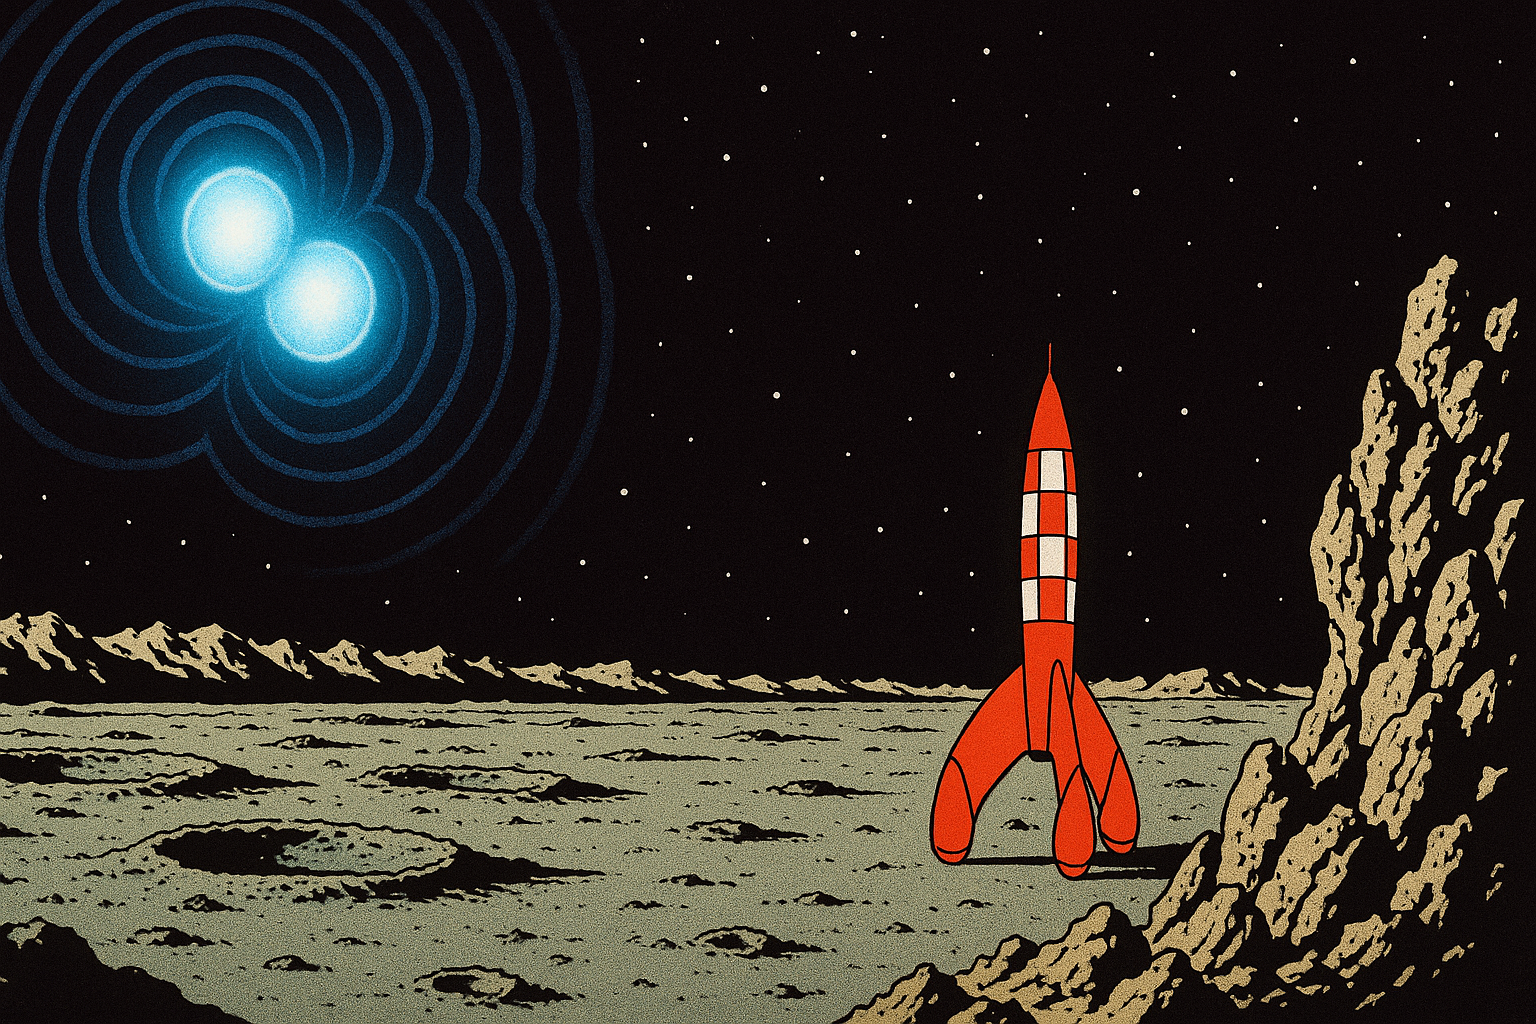
\includegraphics[width=\paperwidth,height=\paperheight]{Figures/tintin_BNS_2.png}}}

\begin{frame}[plain, noframenumbering]

  \begin{tikzpicture}[remember picture,overlay]
    \node[fill=customblue, fill opacity=0.75, text opacity=1, rounded corners=10pt, inner sep=15pt] at (current page.center) {
      \begin{minipage}{0.8\textwidth}
        \centering
        \textbf{Towards GPU-accelerated multimessenger inference of neutron star mergers and dense matter physics}\\[1.5ex]
        \normalsize Thibeau Wouters \\[0.5ex]
        \github \quad \linkedin \quad \myemail
      \end{minipage}
    };
  \end{tikzpicture}
  
  \vspace{7cm}

  \begin{columns}
  \column{0.35\textwidth}
  \begin{figure}
    \centering
    \vspace{1.5mm}
    
\includegraphics[width=0.75\linewidth]{Figures/utrecht-university.png}
  \end{figure}
  \column{0.35\textwidth}
  \begin{figure}
    \centering
    
\includegraphics[width=0.75\linewidth]{Figures/Nikhef_logo-transparent.png}
  \end{figure}
\end{columns}
  
  \end{frame}
}

% %The next statement creates the title page.
% \frame[plain]{\titlepage
% }


%---------------------------------------------------------
%This block of code is for the table of contents after the title page
% \begin{frame}[plain, noframenumbering]
% \frametitle{Table of Contents}
% \tableofcontents
% \end{frame}
%---------------------------------------------------------

\begin{frame}
\frametitle{Table of Contents}
\tableofcontents[hideallsubsections]
\end{frame}

\section{Introduction}

\subsection{Neutron stars and equation of state}

\begin{frame}{Neutron stars}

  \def\x{3mm}

  \begin{itemize}
    \item Neutron stars: supernova remnants, densest matter in the universe

    \item $m \sim 1.2 - 2.3 M_\odot$, $R \sim 10-13$ km

    \item<2-> Cosmic laboratories for fundamental physics
  \end{itemize}

  \only<1>{
    \centering
    \incfig[0.90\textwidth]{NS_above_Berlin}
  }
  
  \only<2>{
    \vspace{\x}
    \begin{figure}
      \centering
      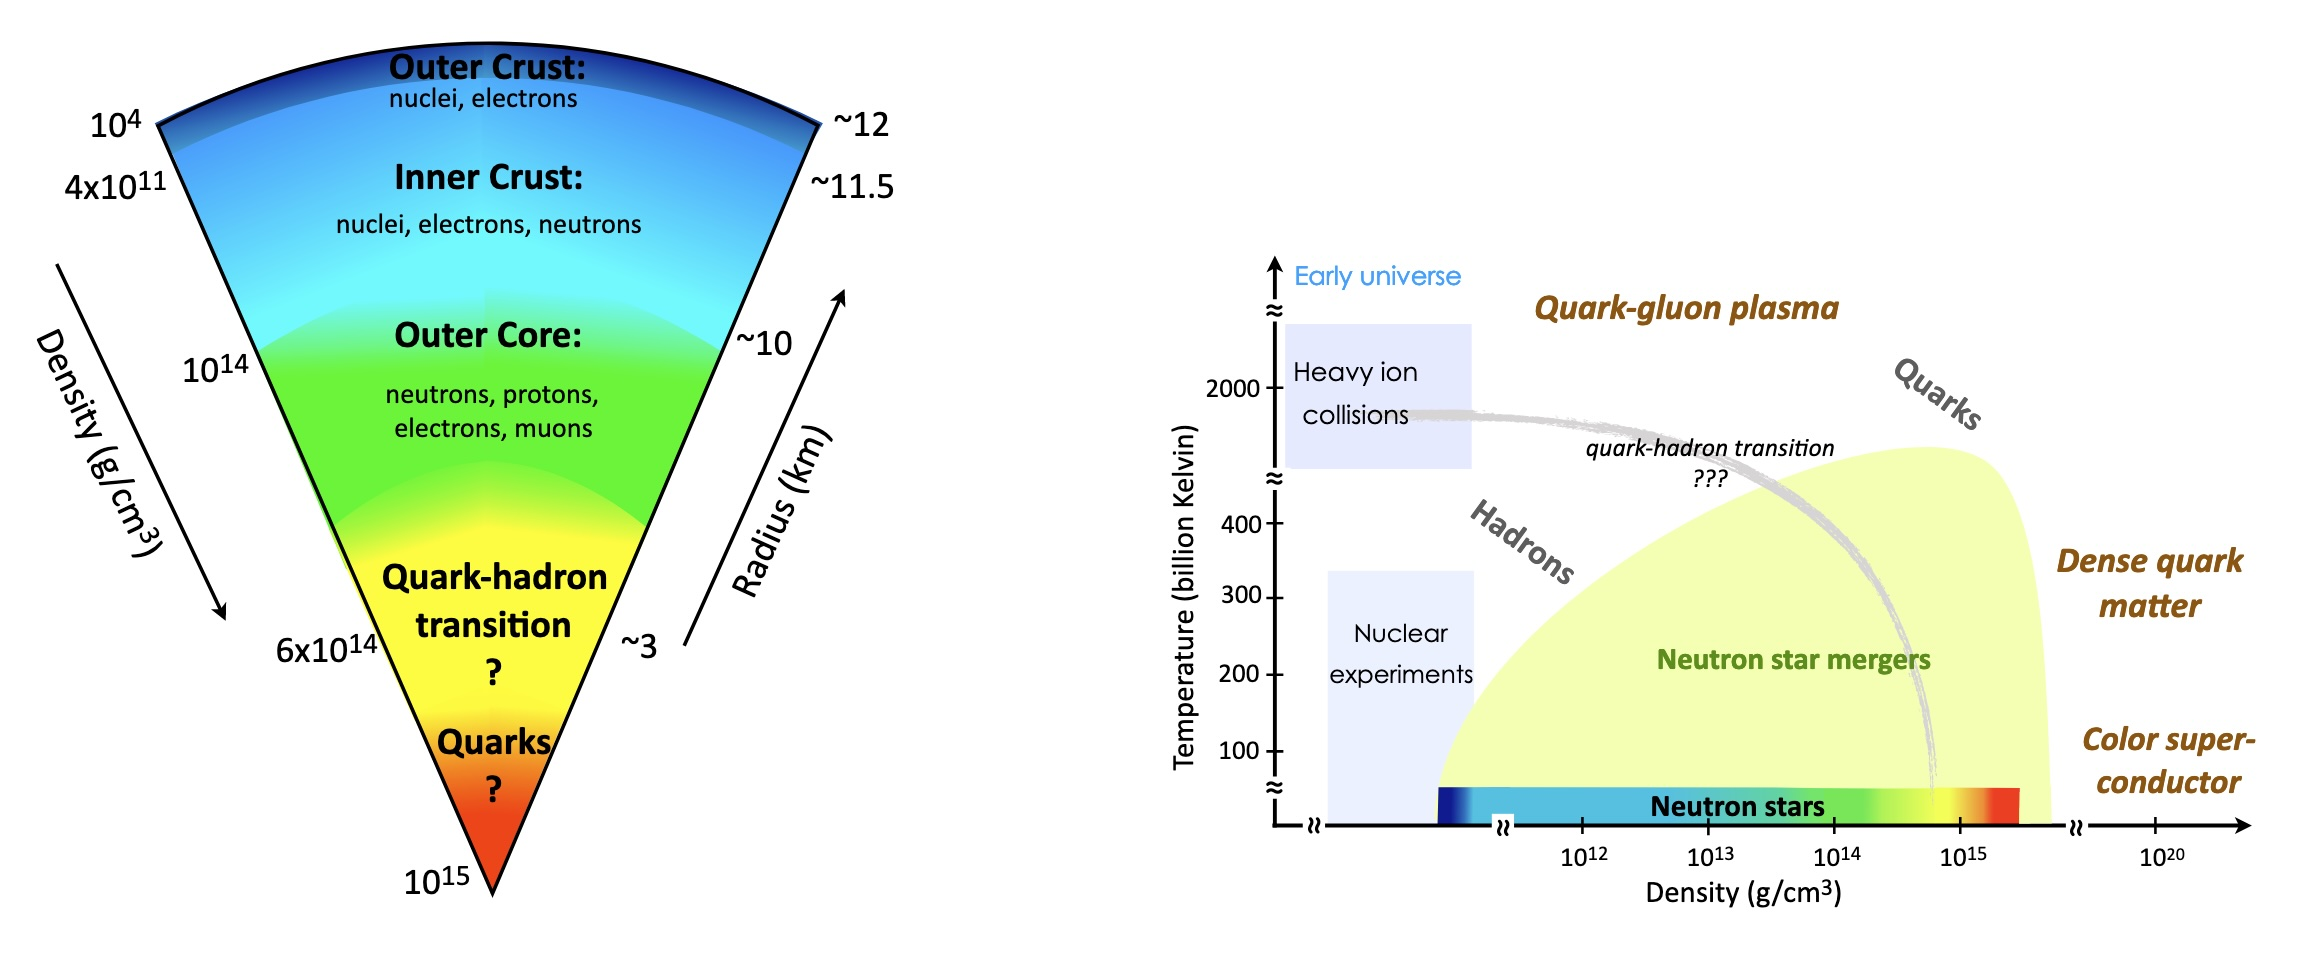
\includegraphics[width=0.99\linewidth]{Figures/NS_diagram.jpg}
    \end{figure}
  }
\end{frame}

\begin{frame}{Equation of state}

  \def\x{3mm}
  \def\y{1mm}

  \begin{itemize}
    \item Neutron stars uniquely probe the cold equation of state (EOS) of dense nuclear matter~\cite{Koehn:2024set}

    \vspace{\y}

    \item How to determine the EOS from neutron stars?
  \end{itemize}

  \vspace{\x}

  \begin{figure}
    \centering
    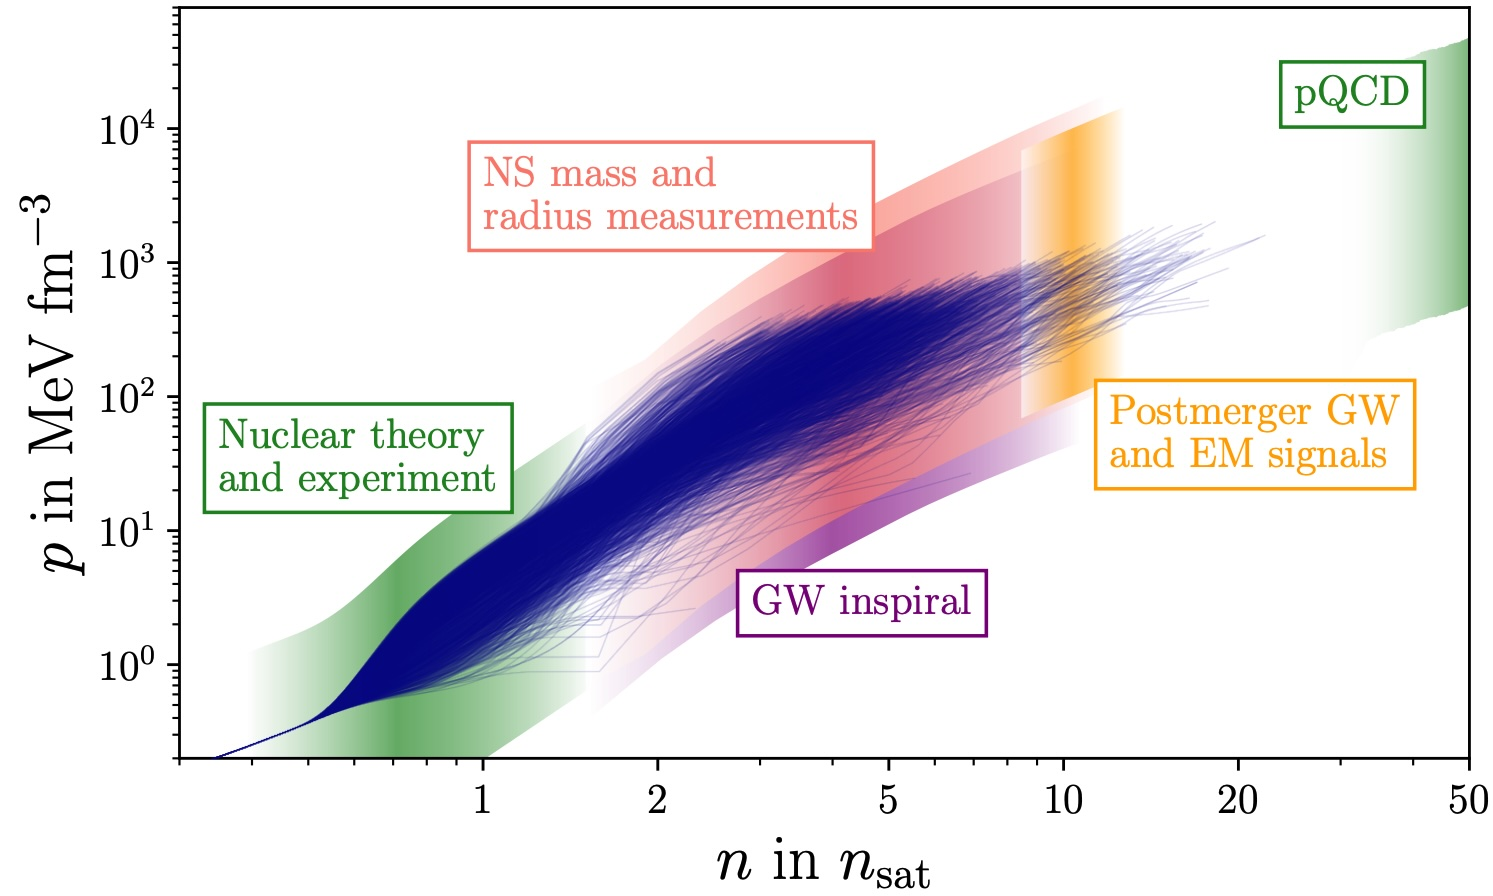
\includegraphics[width=0.80\linewidth]{Figures/Koehn_EOS.jpg}
  \end{figure}
\end{frame}

% \begin{frame}{Neutron star masses}
%   \todo{Fill}
% \end{frame}


% \begin{frame}{Neutron star masses and radii}
%   \todo{Fill}
% \end{frame}


% \begin{frame}{Neutron star masses and tidal deformation}
%   \todo{Fill}
% \end{frame}


\subsection{Multimessenger astrophysics}


\begin{frame}{Multimessenger astrophysics}

  \def\x{2mm}
  
  Observe neutron star mergers through gravitational waves and electromagnetic radiation: GW170817~\cite{LIGOScientific:2017vwq, LIGOScientific:2017zic}

  \todo{Snapshots}
\end{frame}

% \begin{frame}{Gravitational waves}

%   \def\x{2mm}
%   \begin{itemize}
%     \item Gravitational waves offer a new way to probe the physics of black holes and neutron stars

%     \vspace{\x}

%     \item LIGO-Virgo-Kagra collaboration detected \red{218} events in GWTC-4.0~\cite{LIGOScientific:2025slb}
    
%     \vspace{\x}

%     \item So far, 2 binary neutron star mergers: GW170817 and GW190425
%   \end{itemize}

%   \vspace{\x}

%   \begin{figure}
%     \centering
%     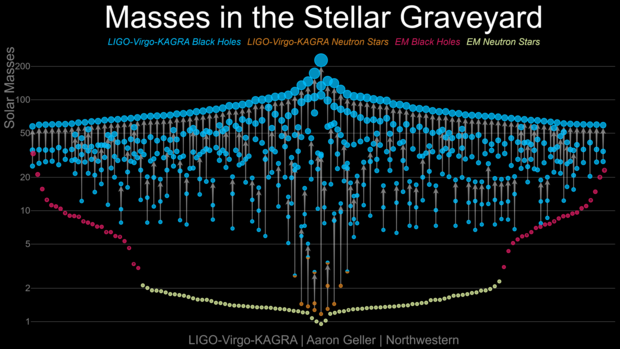
\includegraphics[width=0.75\linewidth]{Figures/stellar_graveyard.png}
%   \end{figure}
% \end{frame}

\begin{frame}{Kilonovae}

  \def\x{3mm}
  \def\y{1mm}

  \begin{itemize}
    \item Electromagnetic counterpart of a binary neutron star merger~\cite{Metzger:2019zeh}

    \vspace{\y}
    
    \item Lasts days-weeks, isotropic
    
    \vspace{\y}

    \item Powered by radioactive decay of heavy elements: r-process
    
    \vspace{\y}

    \item Ejecta depend on EOS \todo{ how and put in the slide}
  \end{itemize}

  \vspace{\x}

  \centering
  \incfig[0.9\textwidth]{KN}
\end{frame}


\begin{frame}{Gamma-ray bursts afterglow}

  \def\x{3mm}
  \def\y{4mm}

  \begin{columns}
    \begin{column}[c]{0.70\textwidth}
      \begin{itemize}
        \item Short gamma-ray burst: relativistic jet launched after merger ($\sim 1$ s)

        \vspace{\y}

        \item Afterglow: broadband emission from radio to X-rays

        \vspace{\y}

        \item Lasts weeks-years
      \end{itemize}
    \end{column}

    \hfill

    \begin{column}[c]{0.25\textwidth}
      \centering
      \incfig[0.75\columnwidth]{GRB_intro}
    \end{column}
  \end{columns}
\end{frame}

% \begin{frame}{Binary neutron star mergers: implications}

%   \def\x{2mm}
  
%   \begin{itemize}
%     \item \textbf{Equation of state}
    
%     \vspace{\x}
    
%     \item Formation site of heavy elements
    
%     \vspace{\x}
    
%     \item Determine Hubble constant

%     \vspace{\x}
    
%     \item Confirm GWs travel at speed of light ($\sim 10^{-15}$)
    
%     \vspace{\x}
    
%     \item<2-> After 10 years of detections: \red{$1$} event
%   \end{itemize}
% \end{frame}

\subsection{Future detectors and challenges}

\begin{frame}{Future GW detectors: Einstein Telescope}
  \def\x{3mm}
  \def\y{2mm}
  \def\z{1mm}

  \red{Einstein Telescope}: Third-generation ground-based GW detector~\cite{ET:2019dnz, Abac:2025saz}
  \begin{itemize}
    \item<2-> Increased sensitivity
    
    \begin{itemize}
      \item Louder signals
      
      \vspace{\z}

      \item $10^{5} - 10^{6}$ black hole mergers/year (now: $\sim 200$/10 years)
      
      \vspace{\z}
      
      \item $10^{4} - 10^{5}$ binary neutron star mergers/year (now: $2$/10 years)

      \vspace{\z}
      
      \item $10^{2} - 10^{3}$ multimessenger events/year (now: $1$/10 years)
    \end{itemize}

    \vspace{\y}

    \item<3-> Observe from $5$ Hz (now: $20$ Hz)
    \begin{itemize}
      \item Longer signals: binary neutron star: $2$ hours vs 2 minutes 
      \item Signals will overlap
    \end{itemize}

    \vspace{\y}

    \item<4-> Can we handle this computationally?
  \end{itemize}
\end{frame}

\begin{frame}{Computational burden of Einstein Telescope}

  \vspace{-5mm}

  \begin{figure}
    \centering
    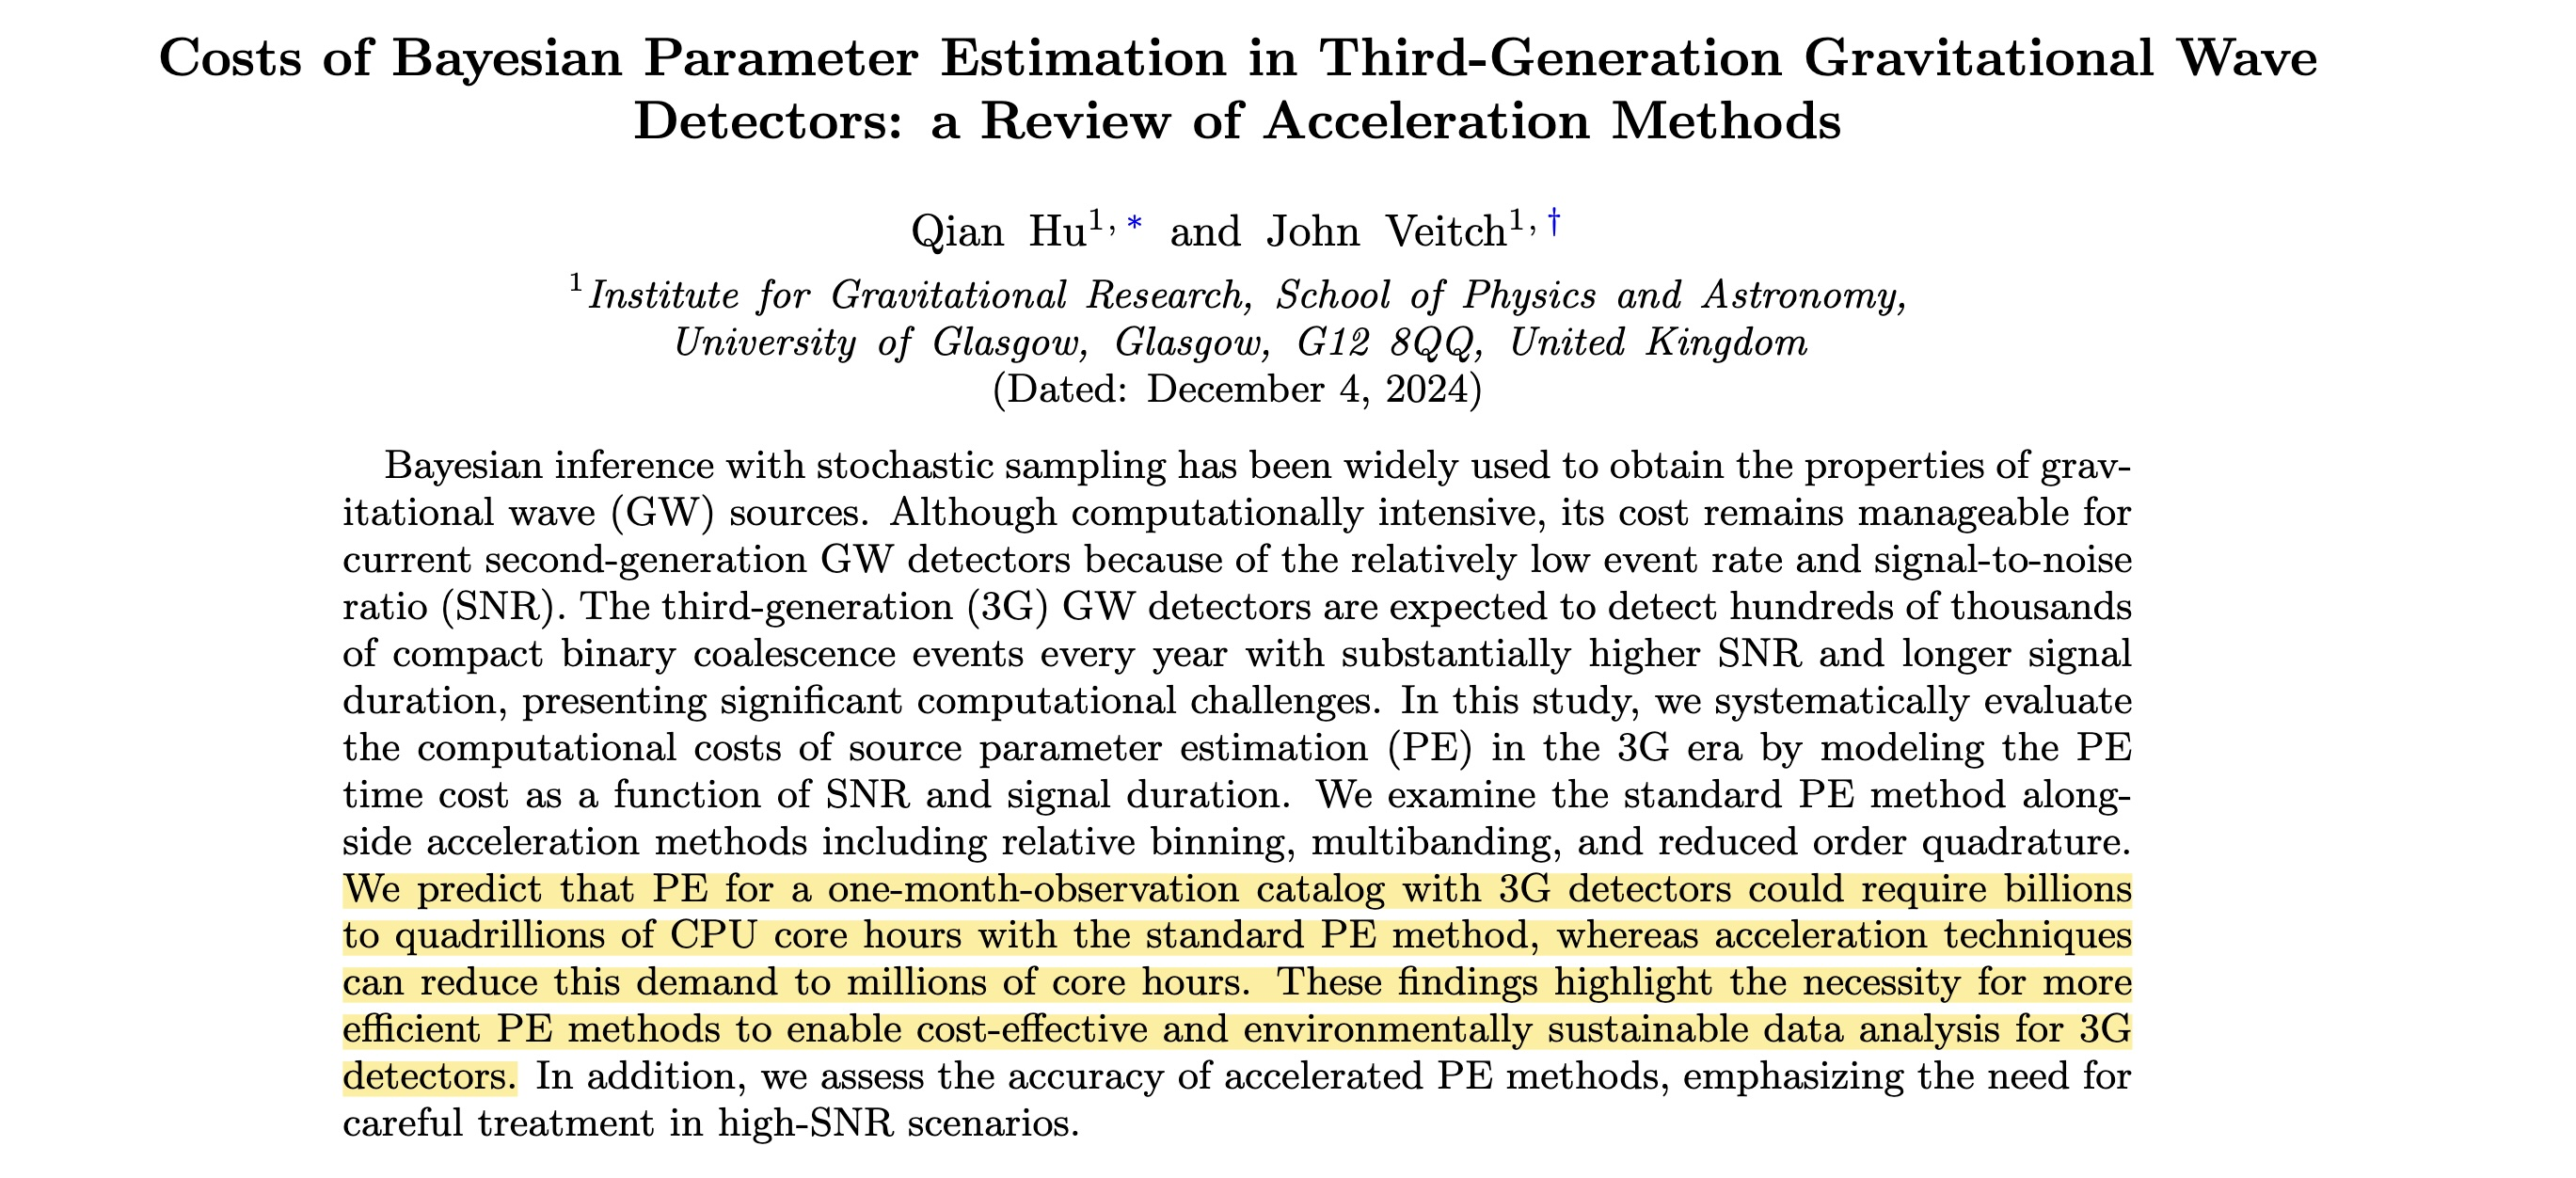
\includegraphics[width=0.95\linewidth]{Figures/Hu_Veitch.jpg}
  \end{figure}

  \vspace{2mm}

  \begin{itemize}
    \item Billions -- quadrillions of CPU hours for 1 month of data~\cite{Hu:2024mvn}

    \item Neglecting binary neutron stars \& multimessenger, overlapping signals,...

    \item \red{Current software does not scale}
  \end{itemize}
\end{frame}

\begin{frame}{My research focus: why -- how -- what}
  \def\x{4mm}
  \def\y{1mm}

  \textbf{Why?}

  To make inference of multimessenger astrophysics scalable

  \begin{itemize}
    \vspace{\y}
    \item Prepare for future detectors

    \vspace{\y}
    
    \item Understand systematic effects through simulated data
  \end{itemize}

  \vspace{\x}
  \pause

  \textbf{How?} 

  Without compromises to flexibility and accuracy

  \begin{itemize}
    \vspace{\y}
    \item Accelerate with GPU hardware, differentiable programming

    \vspace{\y}

    \item Use machine learning to assist inference, not replace it
  \end{itemize}

  \vspace{\x}
  \pause

  \textbf{What?}

  GPU-accelerated Bayesian joint inference framework of neutron star mergers and dense matter physics
\end{frame}


\section{Methods}

\subsection{Bayesian inference and sampling}

\begin{frame}{Parameter estimation: Bayesian inference}

  \def\x{3mm}

  How do we ``measure'' source parameters $\theta$ for data $d$? 

  \vspace{\x}
  
  Bayesian inference:
  \begin{equation*}
    {\rm{posterior}} = p(\theta|d, \mathcal{M}) = \frac{p(d|\theta, \mathcal{M}) p(\theta | \mathcal{M})}{p(d | \mathcal{M})} = \frac{\rm{likelihood} \times \rm{prior}}{\rm{evidence}}
  \end{equation*}

  \begin{itemize}
    \item Prior: specified by users
    
    \item Likelihood: often costly
    
    \item Posterior: intractable, needs stochastic samplers

    \item Evidence: model selection
  \end{itemize}
\end{frame}

\begin{frame}{Parameter estimation: Nested sampling}

  \def\x{3mm}

  How do we sample the posterior? \red{Nested sampling}

  \todo{explain nested sampling}
\end{frame}

\begin{frame}{Parameter estimation: Markov chain Monte Carlo}

  \def\x{3mm}

  How do we sample the posterior? \red{Markov chain Monte Carlo}

  \begin{itemize}
    \item $N$ chains $\boldtheta_i$ sample posterior in parallel
    
    \item Evolve chains to new position: proposal 
    
    \item Compute likelihood $\rightarrow$ \mcmcgreen{accept}/\mcmcred{reject}
  \end{itemize}

  \vspace{\x}

  \centering
  \incfig[0.9\textwidth]{sampling}
\end{frame}

\begin{frame}{Computational aspects}

  \def\x{3mm}
  \def\y{1mm}

  \begin{equation*}
    {\rm{Total \ runtime}} \approx \red{N_{{\rm{likelihood}}}} \times \blue{\tau_{{\rm{likelihood}}}}
  \end{equation*}

  \pause

  \begin{itemize}
    \item $\red{N_{{\rm{likelihood}}}}$:
    \begin{itemize}
      \item Dimensionality of $\boldtheta$
      
      \vspace{\y}
      
      \item Signal-to-noise ratio
      
      \vspace{\y}
      
      \item Multimodality/shape posterior
      
      \vspace{\y}

      \item Efficiency of sampler (proposals)
    \end{itemize}

    \vspace{\x}
    \pause

    \item $\blue{\tau_{{\rm{likelihood}}}}$:
    \begin{itemize}
      \item Complexity model

      \vspace{\y}

      \item Parallelization of likelihood evaluations

      \vspace{\y}
      
      \item Hardware
    \end{itemize}
  \end{itemize}
\end{frame}

\begin{frame}{Tidal deformability}
  \def\x{4mm}

  \begin{itemize}
    \item Neutron stars are tidally deformed in a binary, quantified by tidal deformability $\Lambda$
    
    \vspace{\x}
    
    \item Depends on the mass and equation of state: $\Lambda = \Lambda(m, \rm{EOS})$
    
    \vspace{\x}

    \item Black holes: $\Lambda = 0$
    
    \vspace{\x}

    \item<2-> Affect phase of GWs
  \end{itemize}

  \only<1>{
    \centering
    \incfig[1.0\textwidth]{tidal}
  }
  \only<2>{
    \centering
    \todo{waveform}
  }
\end{frame}

\begin{frame}{Neutron star observables}

  \def\x{2mm}
  
  \begin{itemize}
    \item Masses, radii, and tidal deformation of neutron stars

    \vspace{\x}

    \item Uniquely determined by the equation of state, have to solve the TOV equations
    
    \vspace{\x}

    \item How can we probe them in multimessenger astronomy?
  \end{itemize}

  \centering
  \incfig[0.90\textwidth]{TOV}
\end{frame}

\begin{frame}{Parameter estimation}
  \def\x{3mm}
  \def\y{3mm}
  \def\z{1mm}

  Estimate parameters $\theta$ of a model for data $d$ with Bayesian inference:
  \begin{align*}
    p(\theta|d) &\propto p(d|\theta) p(\theta) \\
    \rm{posterior} &\propto \rm{likelihood} \times \rm{prior}
  \end{align*}

  \pause

  \vspace{4mm}

  \begin{itemize}
    \item Sample the posterior: MCMC or nested sampling

    \vspace{\z}

    \item Propose samples, \mcmcgreen{accept}/\mcmcred{reject} based on likelihood

    \vspace{\z}
    
    \item $\mathcal{O}(10^6)$ likelihood evaluations: computational bottleneck
  \end{itemize}
  
  \vspace{2mm}

  \centering
  \incfig[0.95\textwidth]{sampling}
  
\end{frame}

\begin{frame}{Future gravitational wave detectors}
  \def\x{5mm}
  \def\y{1mm}

  Future GW detectors: 10$\times$ more sensitive
  \begin{itemize}
    \item $\mathcal{O}(10^5)$ events/year (now: $\mathcal{O}(10^2)$ events/decade)

    \vspace{\y}
    
    \item Signals are longer, louder, and overlap
  \end{itemize}

  \pause

  \begin{tcolorbox}[colback=blue!10, boxrule=0pt]
    \textbf{Premise}: Current software does not meet these demands~\cite{Hu:2024mvn}
  \end{tcolorbox}

  \pause
  \vspace{\x}

  How to make parameter estimation scalable?
  \begin{itemize}
    \item Reduce cost of likelihood evaluations

    \vspace{\y}

    \item Improve MCMC proposals
  \end{itemize}

  \pause
  \begin{tcolorbox}[colback=blue!10, boxrule=0pt]
    \textbf{Goal}: Fast sampling with minimal pretraining: flexible alternative to simulation-based inference~\cite{Langendorff:2022fzq, Bhardwaj:2023xph, Dax:2024mcn, Hu:2024oen, Santoliquido:2025lot}
  \end{tcolorbox}
  \vspace{\y}
  % \begin{itemize}
  %   \onslide<2->{
  %     \item Simulation-based inference~:
  %     \begin{itemize}
  %       \item[$\boldsymbol{\green{+}}$] Fast at inference ($\sim$seconds)
  
  %       \vspace{\y}
  
  %       \item[$\boldsymbol{\red{-}}$] Needs pre-trained model
  %     \end{itemize}
  %   }

  %   \vspace{\y}

  %   \item \only<4->{\textbf{\blue{Hybrid approach: faster likelihoods + NF proposals $\rightarrow$ this talk}}}%
  %     \only<3>{Hybrid approach: faster likelihoods + NF proposals}
  %     \onslide<3->{

  %     \begin{itemize}
  %       \item[$\boldsymbol{\green{+}}$] No pre-training: more flexibility

  %       \vspace{\y}

  %       \item[$\boldsymbol{\red{-}}$] Re-implement software
  %     \end{itemize}
  %     }
  % \end{itemize}

\end{frame}

% \begin{frame}{Towards scalable inference}
%   \def\x{5mm}
%   \def\y{1mm}

  
%   \end{itemize}

%   % \vspace{2mm}
%   % \textbf{\blue{This talk focuses on the hybrid approach}}
% \end{frame}

% \begin{frame}{Normalizing flows (NFs)}
%   \def\x{2mm}

%   \begin{itemize}
%     \item Trainable bijection between \blue{latent} and \red{data} spaces

%     \vspace{\x}
    
%     \item Sample and evaluate complicated densities

%     % \vspace{\x}
    
%     % \item Used as \red{proposal distribution}, trained from MCMC chains
%   \end{itemize}

%   \centering
%   \incfig[0.90\textwidth]{NF}
% \end{frame}

\begin{frame}{\textsc{Jax} \& \textsc{flowMC} \small (Kaze Wong) \normalsize}

  \begin{columns}
    \begin{column}{0.84\linewidth}
      Accelerate Python with \textsc{Jax}~\ghlink{jax-ml/jax}:
      \begin{itemize}
        \item GPUs
        \item Automatic differentiation:
        \begin{itemize}
          \item Gradient-based samplers
          \item Optimization
        \end{itemize}
      \end{itemize}
    \end{column}
    \begin{column}{0.15\linewidth}
      \begin{figure}
        \centering
        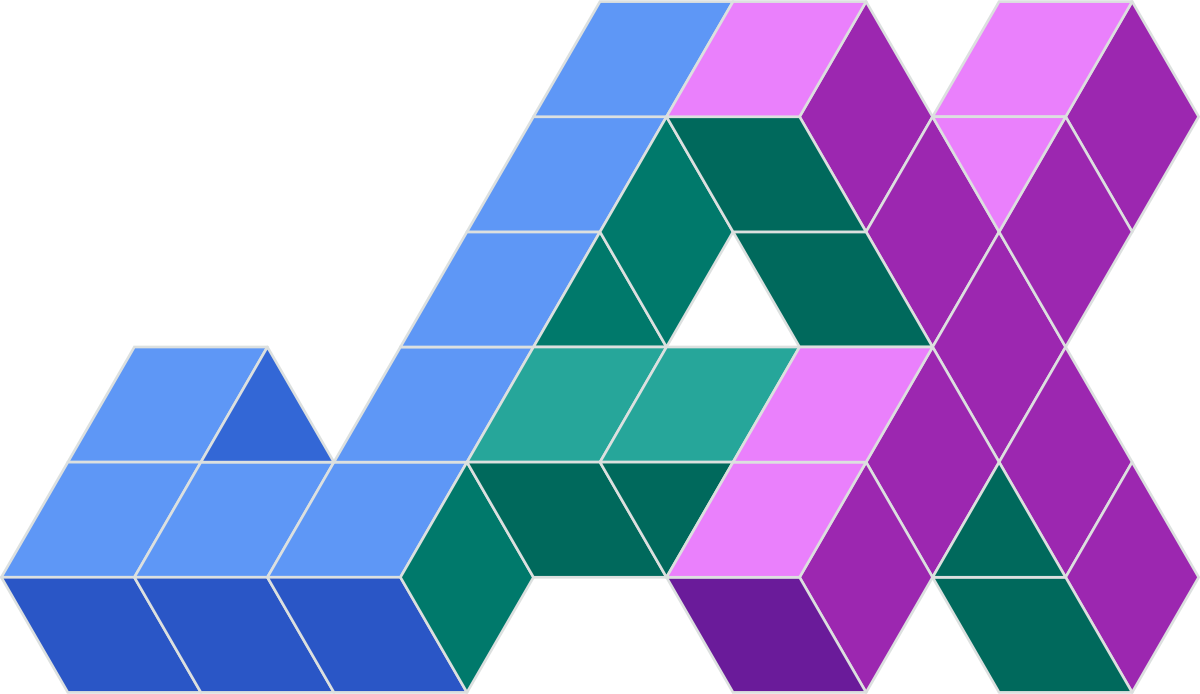
\includegraphics[width=0.95\linewidth]{Figures/jax.png}
      \end{figure}
    \end{column}
  \end{columns}

  \pause
  \vspace{6mm}

  \textsc{flowMC}~\ghlink{kazewong/flowMC}~\cite{Gabrie:2021tlu, Wong:2022xvh}:
  \begin{itemize}
    \item MCMC + normalizing flow proposals in \textsc{Jax}
    \item Training data: MCMC chains $\rightarrow$ \red{no pre-training}
    % \item Use NF as proposal density
    \item<3-> Also see \textsc{nessai}~\ghlink{mj-will/nessai}~\cite{Williams:2021qyt, Williams:2023ppp}, \textsc{pocoMC}~\ghlink{minaskar/pocomc}~\cite{Karamanis:2022ksp}
  \end{itemize}
  \vspace{3mm}

  \centering
  \incfig[0.95\textwidth]{flowMCOverview2}
\end{frame}

\section{Applications}

\begin{frame}{Overview}
  \showoverview{1}
\end{frame}

\begin{frame}{Gravitational waves}
  \def\x{3mm}
  \def\y{5mm}
  \def\z{1mm}

  \vspace{-3mm}
  
  \begin{columns}
    \begin{column}[t]{0.62\linewidth}
      \begin{itemize}
        \item \red{Waveforms} on GPU: $\mathcal{O}(10^3)$ faster

        \vspace{\x}
        
        \item From \textsc{lalsuite} to \textsc{Jax}: \textsc{ripple}~\ghlink{tedwards2412/ripple/}~\cite{Edwards:2023sak}
        \begin{itemize}
          \item Also see \textsc{sfts}~\ghlink{rodrigo-tenorio/sfts}~\cite{Tenorio:2025gci}
        \end{itemize}
      \end{itemize}
    \end{column}

    \begin{column}[t]{0.36\linewidth}
      \begin{figure}
        \centering
        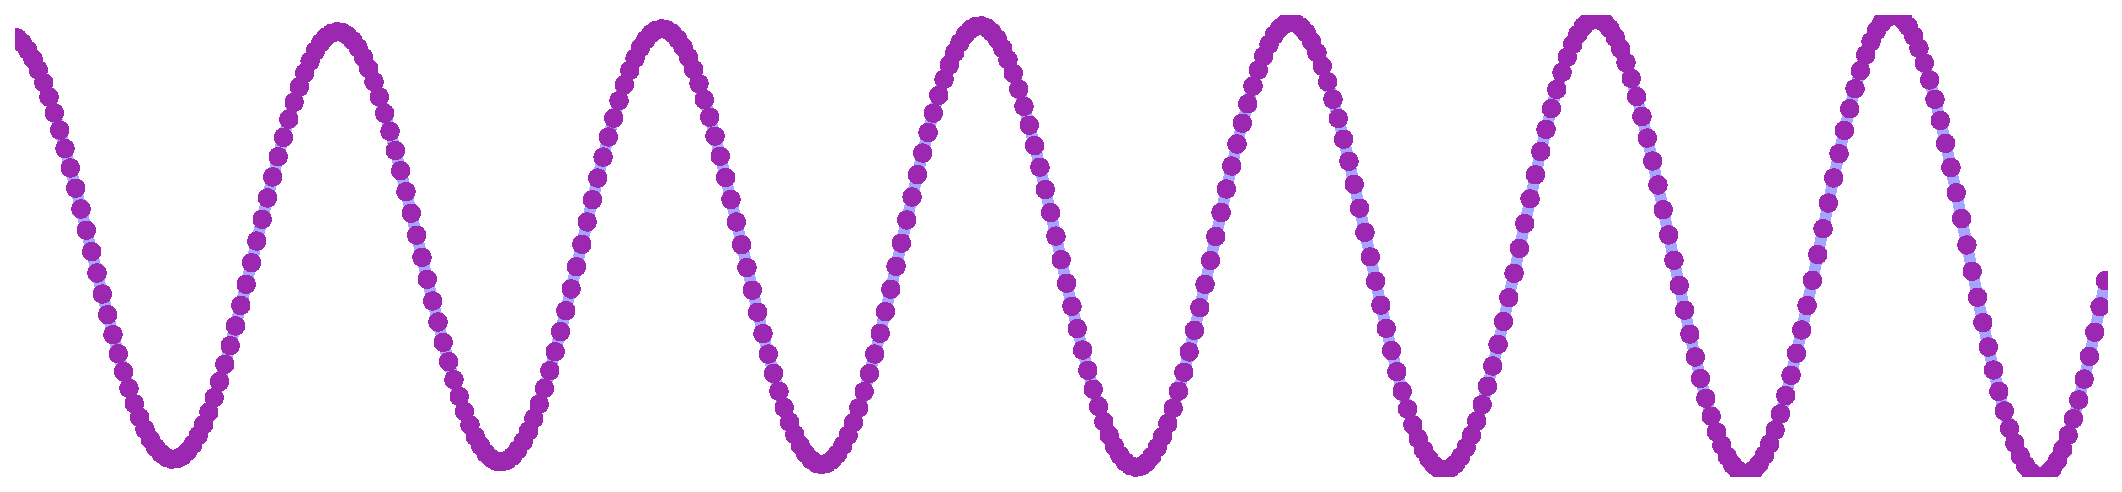
\includegraphics[width=0.99\linewidth]{Figures/strain_zoomed.pdf}
      \end{figure}
    \end{column}
  \end{columns}

  \pause

  \vspace{5mm}
  \hrule
  \vspace{2.5mm}

  \begin{columns}
    \begin{column}[t]{0.60\linewidth}
      \begin{itemize}
        \item \red{Parameter estimation}: \textsc{Jim}~\ghlink{kazewong/jim}~\cite{Wong:2023lgb,Wouters:2024oxj}
    
        \vspace{\x}
    
        \item \green{\checkmark} Current detectors
        \begin{itemize}
          \item Hours $\rightarrow$ minutes
        \end{itemize}
    
        \vspace{\x}

        \onslide<3->{
        \item Ongoing work for future detectors:
        \begin{itemize}
          \item Binary neutron star: 13D

          % \vspace{\z}

          % \item $f_{\rm{min}} = 20$ Hz, SNR = $21$

          \vspace{\z}
          
          \item Einstein Telescope
          
          % \vspace{\z}
          
          % \item \texttt{IMRPhenomD\_NRTidalv2}

          \vspace{\z}

          \item \red{30 mins} on H100 GPU
        \end{itemize}

        % \vspace{\x}

        % \item Evidence? \textsc{harmonic}~\cite{Polanska:2024zpn}
        }
      \end{itemize}
    \end{column}

    \onslide<3->{
    \begin{column}[t]{0.39\linewidth}
      \begin{figure}
        \centering
        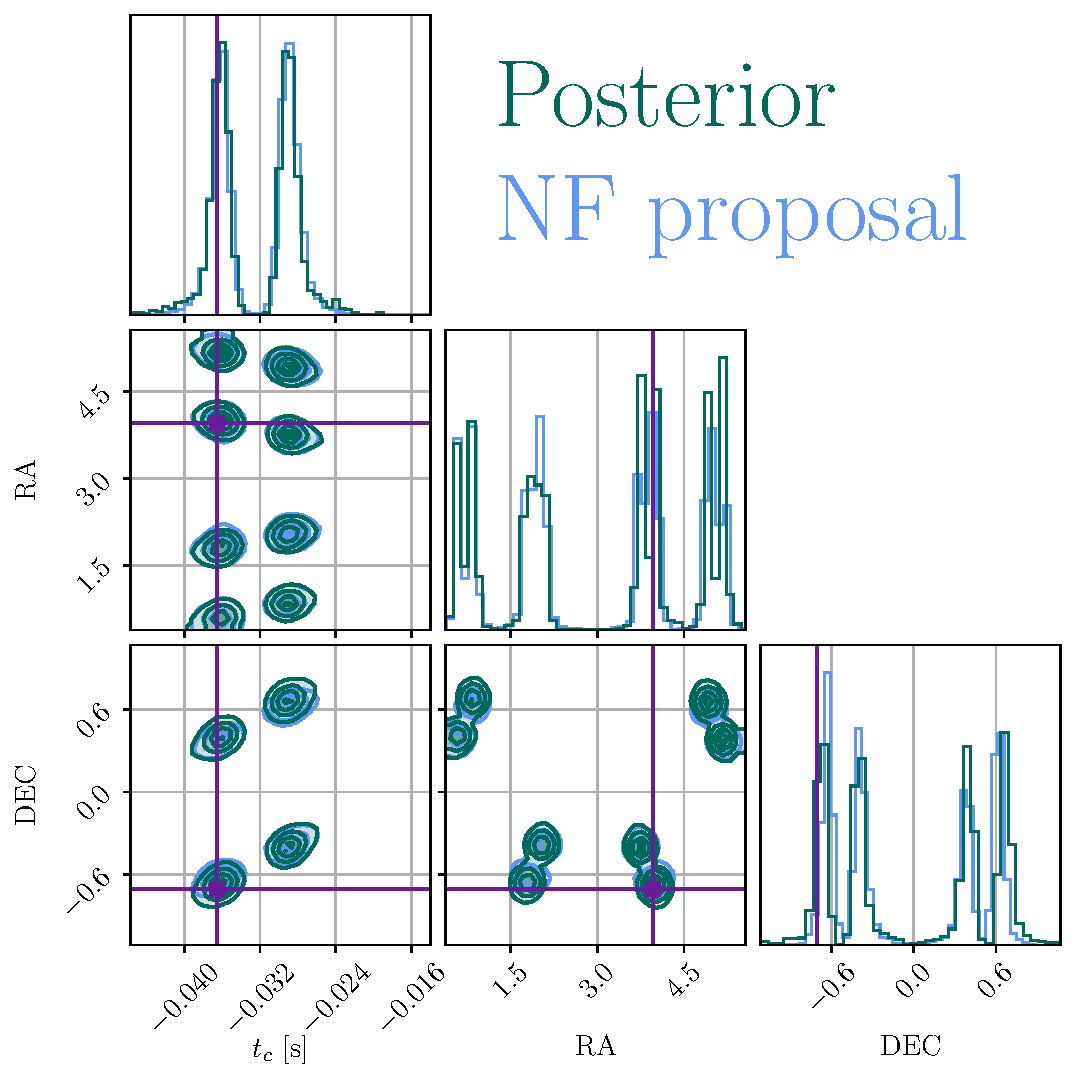
\includegraphics[width=0.99\linewidth]{Figures/corner_plot.pdf}
      \end{figure}
    }
    \end{column}
  \end{columns}
\end{frame}

\begin{frame}{Overlapping signals \tiny (Luca Negri, Justin Janquart, James Alvey, Uddipta Bhardwaj) \normalsize}

  \def\x{1mm}

  %%% Colors used in case needed later on?
  % JAX_BLUE = "#2a56c6" # jax blue, darker
  % JAX_GREEN = "#00695c" # jax green, darker
  % JAX_PURPLE = "#6a1b9a" # jax purple, darker

  % https://github.com/ThibeauWouters/jim_testing/tree/9ff1d374c3fa50f95ded8c2446a579c5f22cbb52/overlapping/HLV_BBH_BBH/outdir/injection_139_v2

  %%% For injection_139_v2, the parameters are: 
  % M_c_1 = 32.06485311503819, M_c_2 = 33.41456227648163

  \begin{itemize}
    % \item In 3G, we expect to see \red{overlapping signals}
    
    \item Assess scaling of \textsc{Jim}: \jaxbluedark{BBH}+\jaxgreendark{BBH} with LIGO-Virgo
    \begin{itemize}
      \vspace{\x}
      \item 2 binary black hole mergers: $22$ parameters

      \vspace{\x}

      \item $\jaxbluedark{M_c^{(1)}} = 32 M_\odot$, $\jaxgreendark{M_c^{(2)}} = 33 M_\odot$, $\Delta t = 70$ ms
      
      \vspace{\x}

      \item $\jaxbluedark{\rm{SNR}^{(1)}} = 25.76$, $\jaxgreendark{\rm{SNR}^{(2)}} = 25.24$ 

      \vspace{\x}

      \item<2-> \red{$1$h$28$m} on H100 (vs 23 days on 16 CPUs~\cite{Janquart:2022fzz})
    \end{itemize}
  \end{itemize}

  \pause

  \onslide<2->{

    \vspace{-4mm}
    
    \begin{columns}
      \begin{column}{0.49\textwidth}
        \begin{figure}
          \centering
          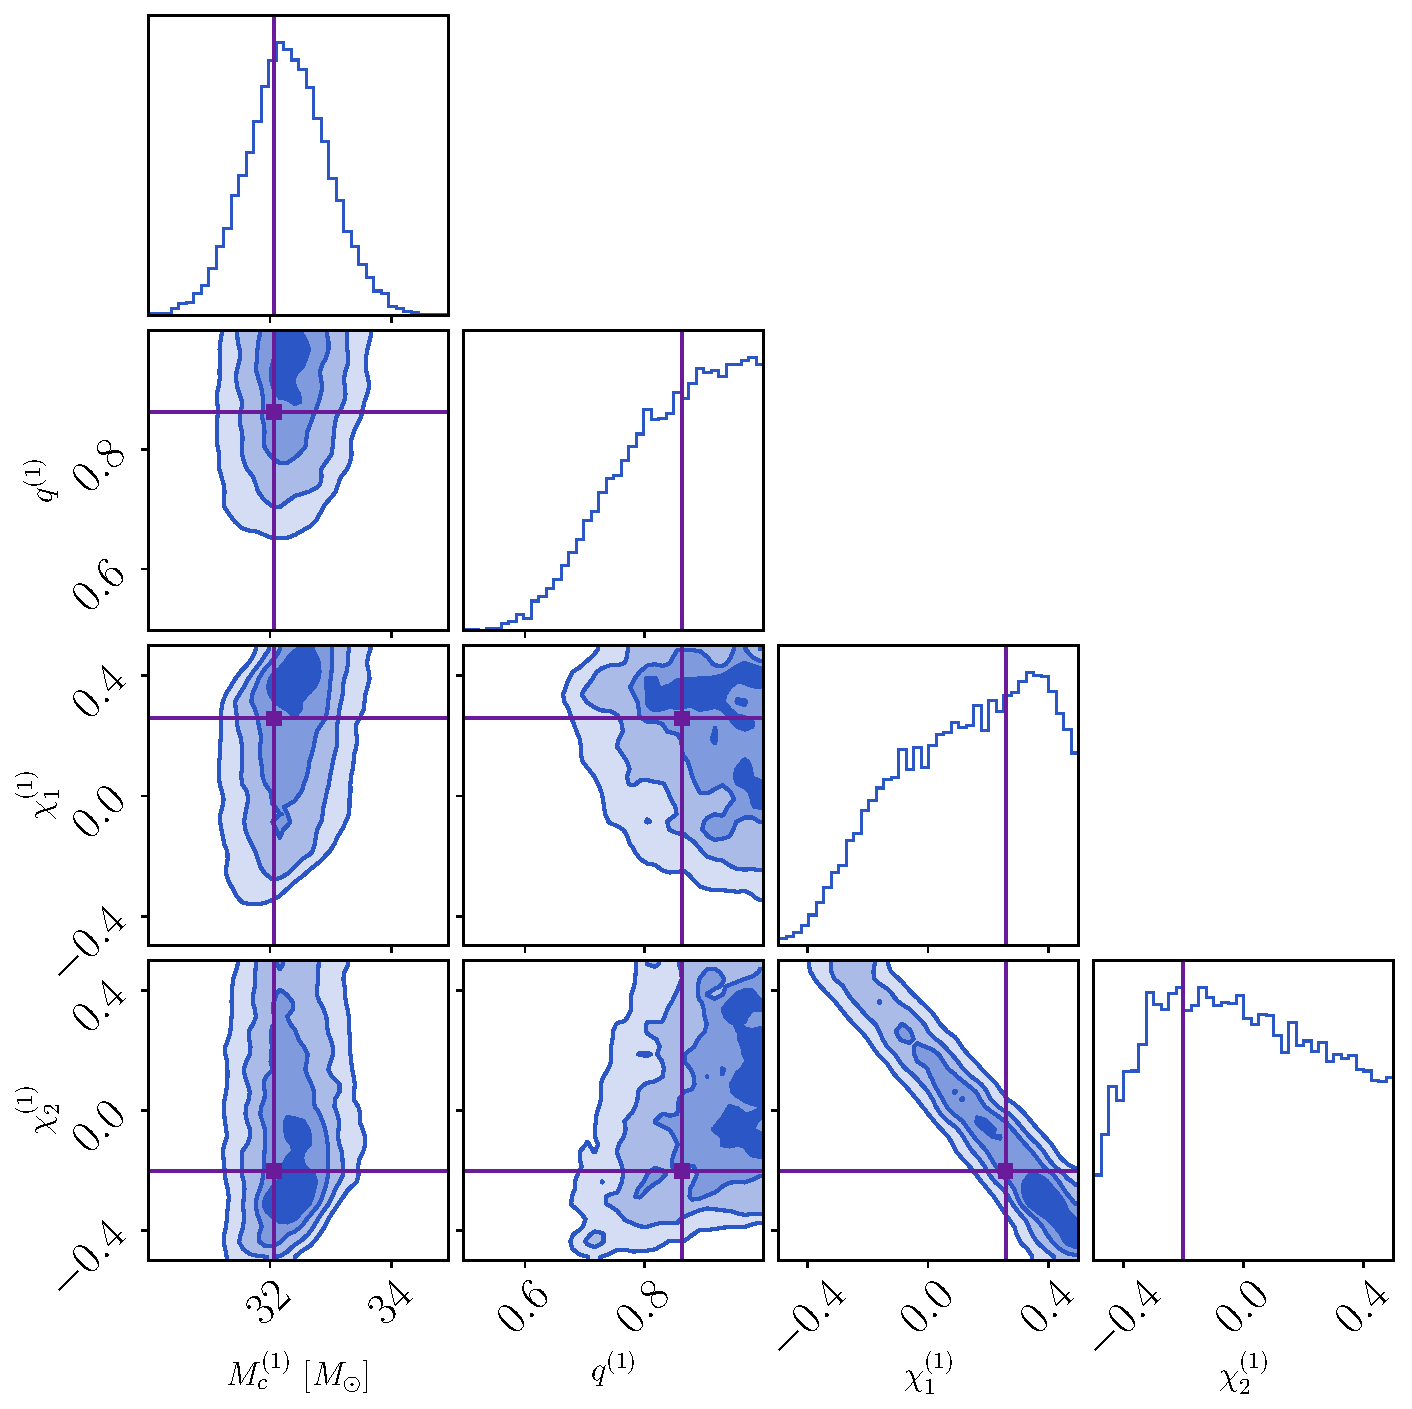
\includegraphics[width=0.85\linewidth]{Figures/OS_injection_139_v2_1_cornerplot_M_c_q_s1_z_s2_z.pdf}
        \end{figure}
      \end{column}

      \begin{column}{0.49\textwidth}
        \begin{figure}
          \centering
          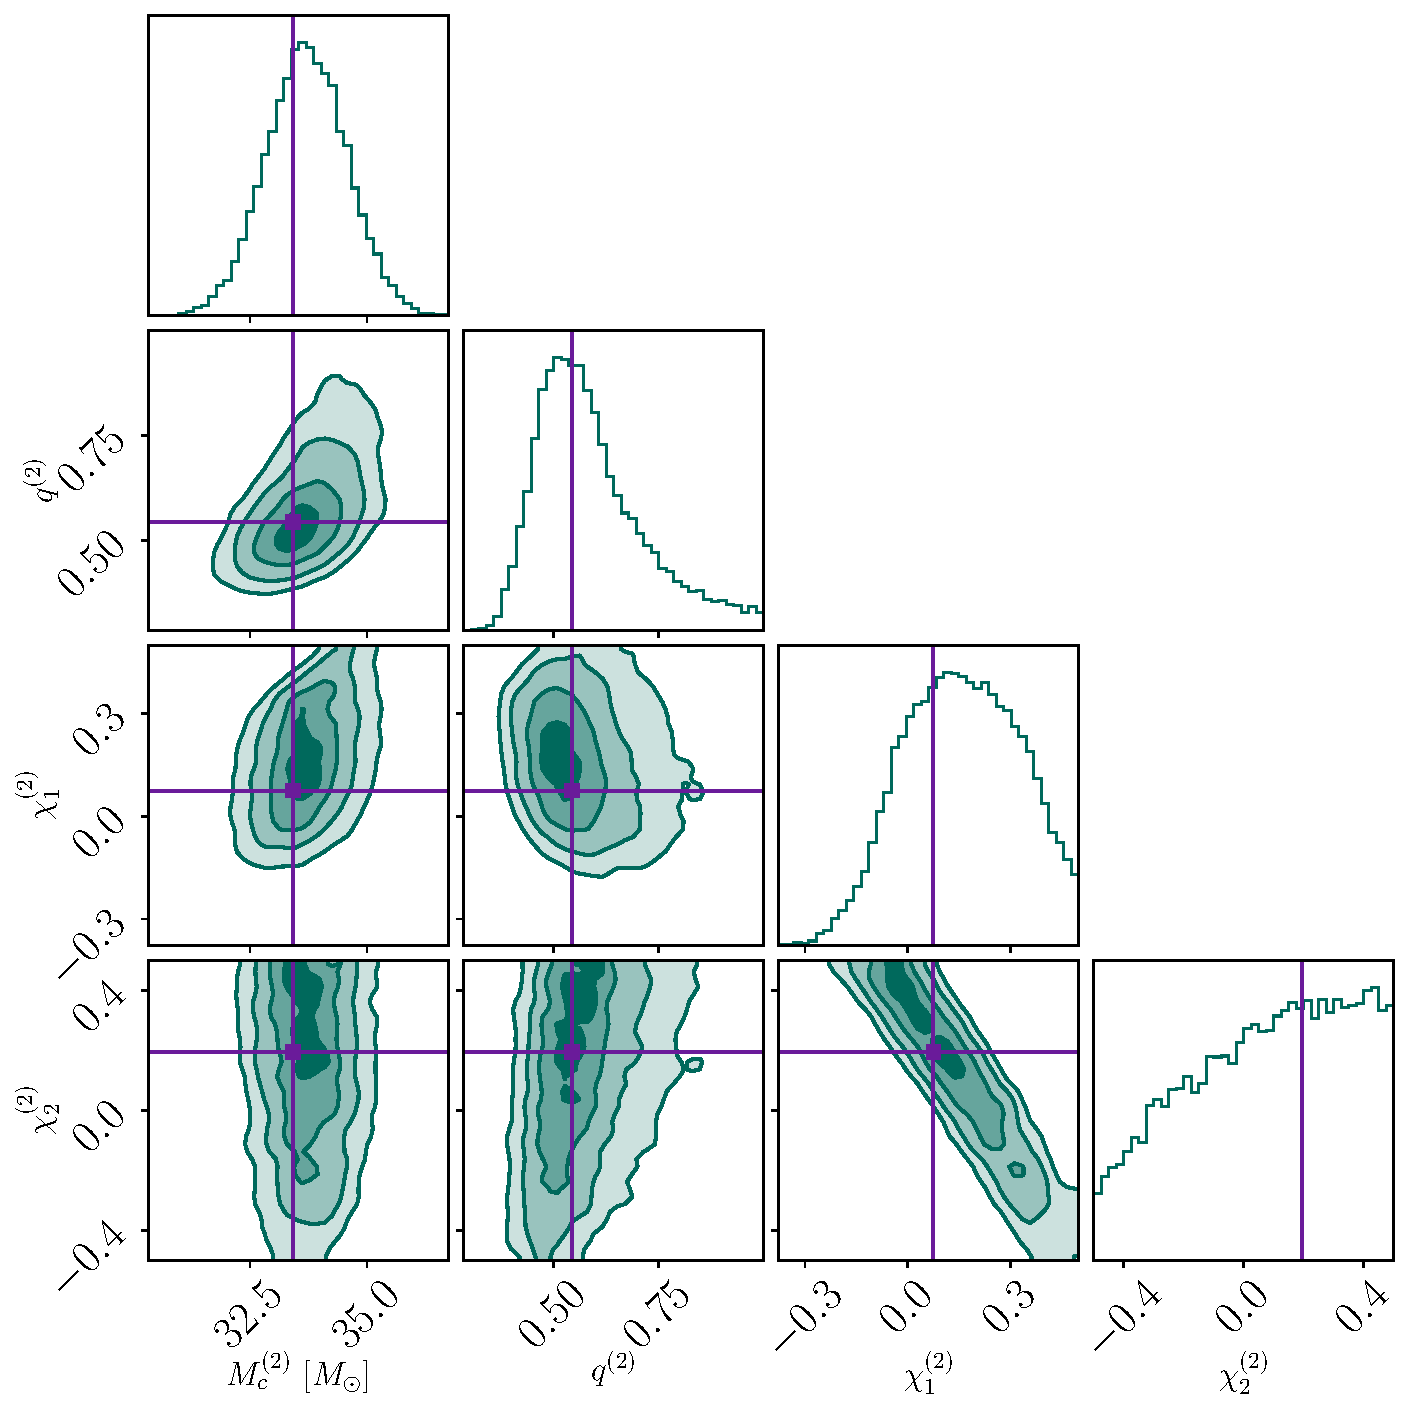
\includegraphics[width=0.85\linewidth]{Figures/OS_injection_139_v2_2_cornerplot_M_c_q_s1_z_s2_z.pdf}
        \end{figure}
      \end{column}
    \end{columns}
  }
\end{frame}

\begin{frame}[plain, noframenumbering]{Overview}
  \showoverview{3}
\end{frame}

\begin{frame}{The nuclear equation of state}
  \def\x{2mm}
  \def\y{2mm}

  \begin{itemize}
    \item The equation of state of dense nuclear matter is uncertain~\cite{Koehn:2024set}

    \vspace{\x}
    
    \item Neutron stars probe its high density regime
    
    \vspace{\x}

    \item Solve inverse problem with Bayesian inference
  \end{itemize}

  \vspace{\x}

  \begin{figure}
    \centering
    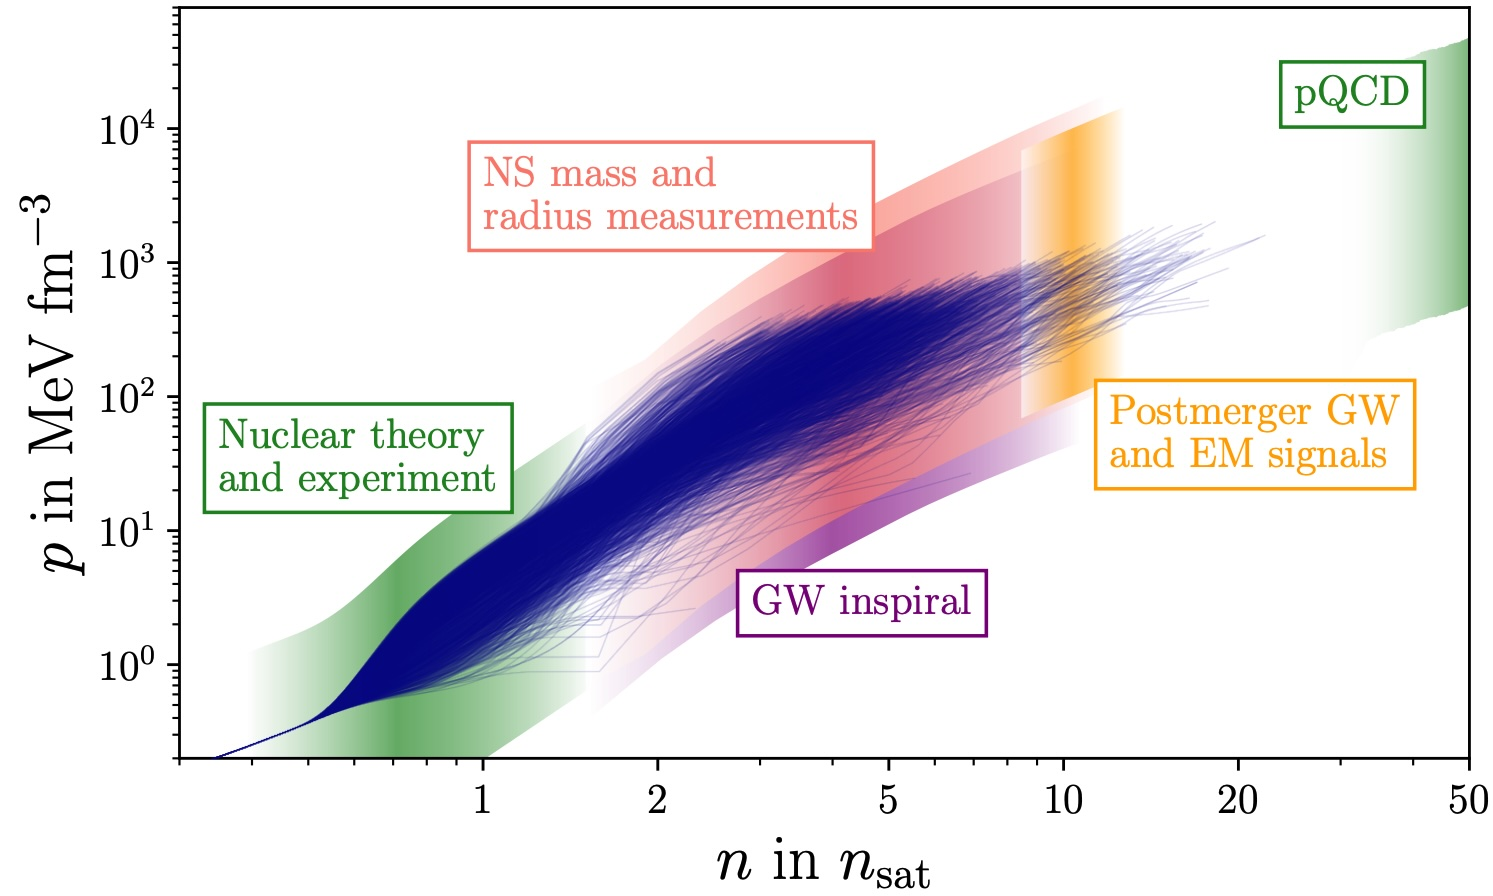
\includegraphics[width=0.75\linewidth]{Figures/Koehn_EOS.jpg} 
  \end{figure}
\end{frame}


\begin{frame}{Equation of state}
  \def\x{2mm}
  \def\y{5mm}

  \begin{itemize}
    \item Parametrization $\theta_{\rm{EOS}}$: constrain with Bayesian inference

    \vspace{\x}

    \item<2-> To predict neutron star properties, we solve the TOV equations: ordinary differential equations (ODEs)
    
    \vspace{\x}

    \item<3-> Done for each sample $\theta_{\rm{EOS}}$: \red{costly likelihood}

    % \vspace{\x}

    % \item Use ML to speed up the process?
  \end{itemize}

  \vspace{\y}

  \only<2>{
    \centering
    \incfig[0.95\textwidth]{TOV}
  }

  \only<3->{
    \centering
    \incfig[0.95\textwidth]{NS_likelihood}
  }

\end{frame}

\begin{frame}{\textsc{Jester} \small (Peter T.H. Pang) \normalsize}
  \def\x{2mm}

  \begin{itemize}
    % \item Goal: infer nuclear equation of state (EOS) of neutron stars~\cite{Abac:2025saz}

    % \vspace{\x}

    \item Solving TOV equations (EOS $\rightarrow$ NS) is slow

    \vspace{\x}

    \item<2-> \textsc{Jester}~\ghlink{nuclear-multimessenger-astronomy/jester}~\cite{Wouters:2025zju}: \textsc{Jax}-based TOV solver
    \begin{itemize}
      \item Full inference in \red{$\sim$hours}
      \item No need for ML emulators
    \end{itemize}

    \vspace{\x}

    \item<3-> End-to-end analysis: from gravitational waves of neutron star mergers to the equation of state
    \begin{itemize}
      \item Example: 20 BNS in O5
    \end{itemize}
    % \begin{itemize}
    %   \item $\Lambda_{1.4}$ tidal deformability of $1.4 M_\odot$ NS
    % \end{itemize}
  \end{itemize}

  \vspace{-3mm}

  \begin{columns}
    \onslide<2->{
      \begin{column}{0.49\textwidth}
        \begin{figure}
          \centering
          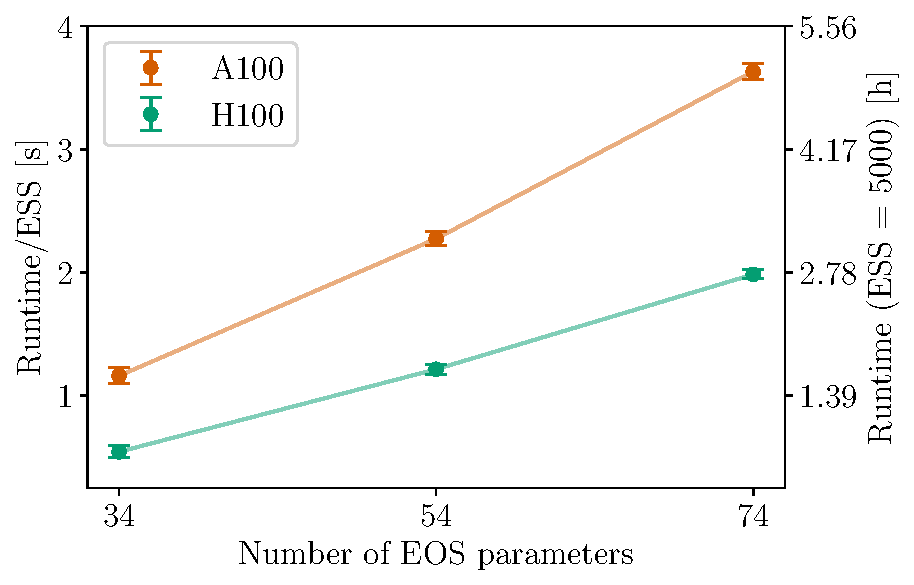
\includegraphics[width=0.99\linewidth]{Figures/scaling_plot.pdf}
        \end{figure}
      \end{column}
    }

    \onslide<3->{
      \begin{column}{0.475\textwidth}
        \begin{figure}
          \centering
          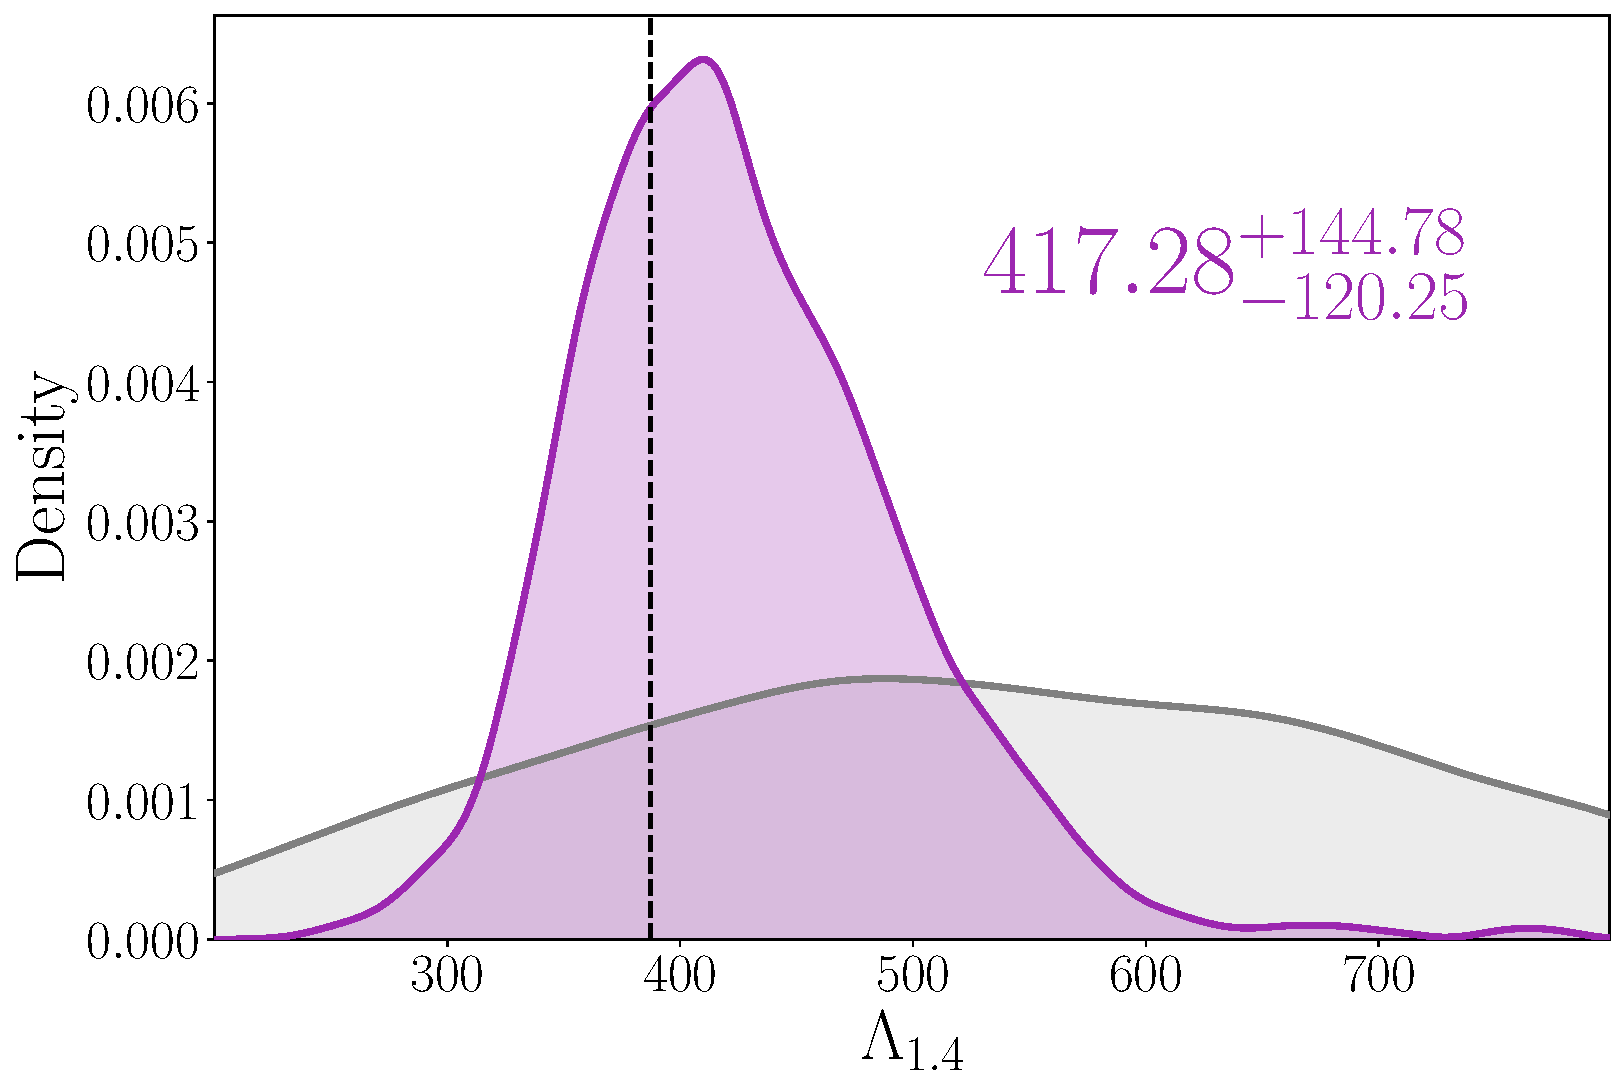
\includegraphics[width=0.99\linewidth]{Figures/BNS_EOS_projection.pdf}
        \end{figure}
      \end{column}
    }
  \end{columns}
\end{frame}

\begin{frame}{Auto-differentiable ODE solvers}

  \def\x{2mm}

  \begin{itemize}
    \item ODE solvers in \textsc{Jax} are auto-differentiable (\textsc{diffrax}~\ghlink{patrick-kidger/diffrax})

    \vspace{\x}

    \item Frame inference as optimization problem:
    \begin{itemize}
      \item Gradient descent on loss function $\mathcal{L}(\theta_{\rm{EOS}})$
    \end{itemize}

    % \vspace{\x}

    % \item<2-> Tool to assess systematics of equation of state inference
  \end{itemize}

  \vspace{3mm}

  \only<2->{
    \centering
    \incfig[0.95\textwidth]{jester_ad}
  }
  
  
\end{frame}

\section{Outlook and conclusion}

\begin{frame}{Conclusion}
  \def\x{4mm}
  \def\y{1mm}

  \begin{itemize}
    \item Progress on scalable Bayesian inference, with minimal pre-training
 
    \vspace{\x}

    \item Hybrid acceleration: GPUs + normalizing flow proposals
    \begin{itemize}
      \vspace{\y}
      \item \textsc{Jax}/GPU: faster likelihoods

      \vspace{\y}

      \item \textsc{flowMC}: sampling converges faster
    \end{itemize}

    \vspace{\x}

    \item Simulators in \textsc{Jax} can remove the need for emulators (GW, TOV)

    \vspace{\x}

    \item Auto-differentiable ODE solvers: inference as optimization problem
  \end{itemize}
  
  \vspace{8mm}

  \textbf{Let's talk!}
\end{frame}

\begin{frame}[plain, noframenumbering]{Thank you for your attention!}

  \def\x{0.5mm}
  
  Software written in \textsc{Jax}~\ghlink{jax-ml/jax}:
  \begin{itemize}
    \vspace{\x}
    \item \textsc{flowMC} \ghlink{kazewong/flowMC}~\cite{Gabrie:2021tlu, Wong:2022xvh}

    \vspace{\x}

    \item \textsc{Jim} \ghlink{kazewong/jim}~\cite{Wong:2023lgb,Wouters:2024oxj} \enumicon{1} \enumicon{2} \enumicon{4}

    \vspace{\x}

    \item \textsc{fiesta} \ghlink{ThibeauWouters/fiestaEM} \enumicon{2} %(work in progress...)

    \vspace{\x}

    \item \textsc{Jester} \ghlink{nuclear-multimessenger-astronomy/jester}~\cite{Wouters:2025zju} (built with \textsc{diffrax}~\ghlink{patrick-kidger/diffrax}) \enumicon{3}

    \vspace{\x}

    \item \textsc{harmonic} \ghlink{astro-informatics/harmonic}~\cite{mcewen2023machinelearningassistedbayesian, polanska2024learnedharmonicmeanestimation, Polanska:2024zpn}
  \end{itemize}

  \centering
  \incfig[0.975\textwidth]{talk_overview}
\end{frame}

\begin{frame}[allowframebreaks]{References}
  \nocite{my_misc_entry}
  \nocite{Kuifje}
  \printbibliography
\end{frame}

\appendix 



\begin{frame}[plain, noframenumbering]{Overview}
  \showoverview{2}
\end{frame}

\begin{frame}{Electromagnetic counterparts \small (Hauke Koehn, Tim Dietrich) \normalsize}
  \def\x{2mm}

  \begin{itemize}
    \item BNS mergers lead to kilonovae, \red{gamma-ray bursts (afterglows)}

    \vspace{\x}
    
    \item Numerical models are expensive (e.g. \textsc{afterglowpy}~\cite{Ryan:2019fhz})
    % \begin{itemize}
      %   \item Kilonovae: \textsc{possis}~\cite{Bulla:2019muo}
      %   \item GRB afterglow: \textsc{afterglowpy}~\cite{Ryan:2019fhz}, \textsc{Pyblastafterglow}~\cite{Nedora:2024vrv}
      % \end{itemize}
      
    \vspace{\x}

    \item<2-> Neural network emulators for inference: \textsc{fiesta}~\ghlink{ThibeauWouters/fiestaEM}
  \end{itemize}

  \onslide<2->{
    \begin{columns}
      \begin{column}[c]{0.14\textwidth}
        \centering
        \incfig[0.90\textwidth]{GRB}
      \end{column}
  
      \begin{column}[c]{0.24\textwidth}

        \vspace{-5mm}

        \fiesta{\textsc{fiesta}}
        \begin{itemize}
          \item $1$m$36$s
          \item $1$ H100 GPU
        \end{itemize}
        
        \vspace{6mm}

        \afterglowpy{\textsc{afterglowpy}}
        \begin{itemize}
          \item $4$ hours
          \item $30$ CPUs
        \end{itemize}
      \end{column}
  
      \begin{column}[c]{0.59\textwidth}
        \begin{figure}
          \centering
          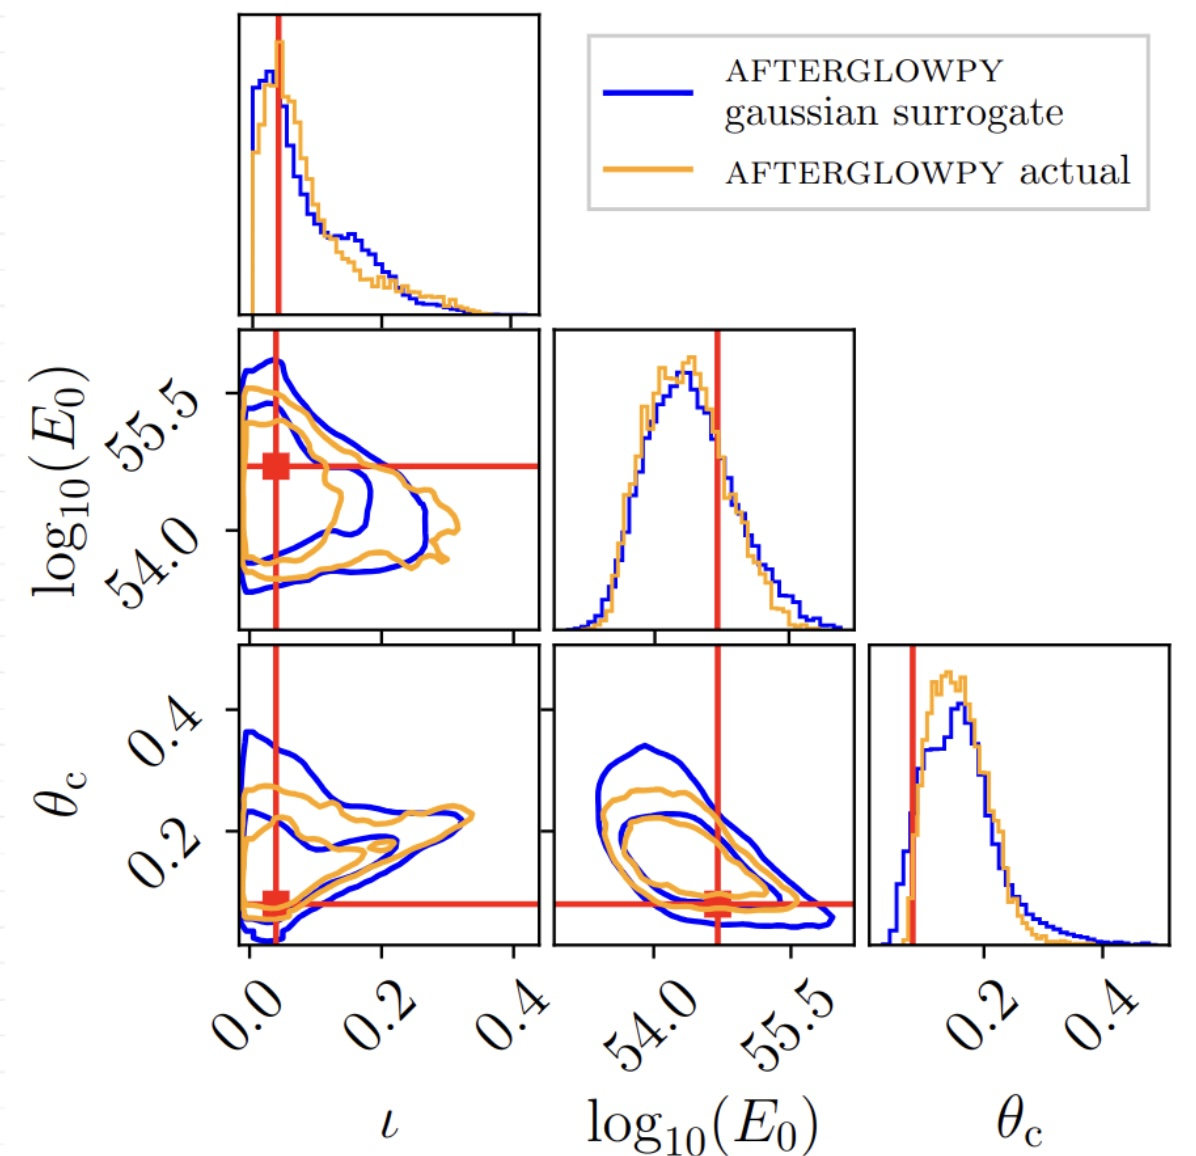
\includegraphics[width=0.80\linewidth]{Figures/fiesta_result.jpg}
        \end{figure}
      \end{column}
    \end{columns}
  }
\end{frame}

\begin{frame}[plain, noframenumbering]{Overview}
  \showoverview{4}
\end{frame}

\begin{frame}{Constructing GWTCs \small (Thomas Ng, Kaze Wong) \normalsize}
  \def\x{2mm}

  GWTCs do not scale well in \red{memory}:
  \begin{itemize}
    \vspace{\x}
    
    \item GWTC stores several samples (different waveforms)
    
    \vspace{\x}
    
    \item Standard: fixed sample size, $\sim 100$ MB

    \vspace{\x}
    
    \item<2-> \textsc{flowMC}: generate samples from normalizing flows, $\sim 10$ MB
    \begin{itemize}
      \item Also see Michael Williams' talk/poster
    \end{itemize}

    % \vspace{\x}

    % \item<3-> Finetune starting from other waveform proposal
  \end{itemize}
  % \begin{itemize}s
  %   \item Importance sampling on NF proposals: generate samples
   
  %   \vspace{\x}
    
  %   \item Finetune on different prior distribution/waveform model
  % \end{itemize}

  \vspace{3mm}

  \centering
  \only<1>{
    \incfig[0.95\textwidth]{GWTC}
  }
  \only<2>{
    \incfig[0.95\textwidth]{GWTC_flowMC}
  }

  % \only<3>{
  %   \incfig[0.95\textwidth]{GWTC_flowMC_finetune}
  % }
  
\end{frame}


% \begin{frame}{Glitch mitigation (Senna van Os, Harsh Narola)}

%   Model glitches as superposition of sine Gaussian wavelets
%   \begin{itemize}
%     \item \textsc{BayesWave}: vary number of wavelets
%     \item \textsc{Jim}: fix $N$ sine Gaussian wavelets, compare different $N$ runs
%     % \item Batch jobs of $N$ wavelets $\rightarrow$ evidence $Z$ $\rightarrow$ Bayes factor
%     % \begin{equation*}
%     %   \ln B_{ij} = \ln Z_i - \ln Z_j
%     % \end{equation*}
%     \item Comparable results to \textsc{BayesWave} 
%     \item $5 \times 10$ mins vs $1h$
%   \end{itemize}

%   \begin{columns}
%     \begin{column}{0.49\textwidth}
%       \begin{figure}
%         \centering
%         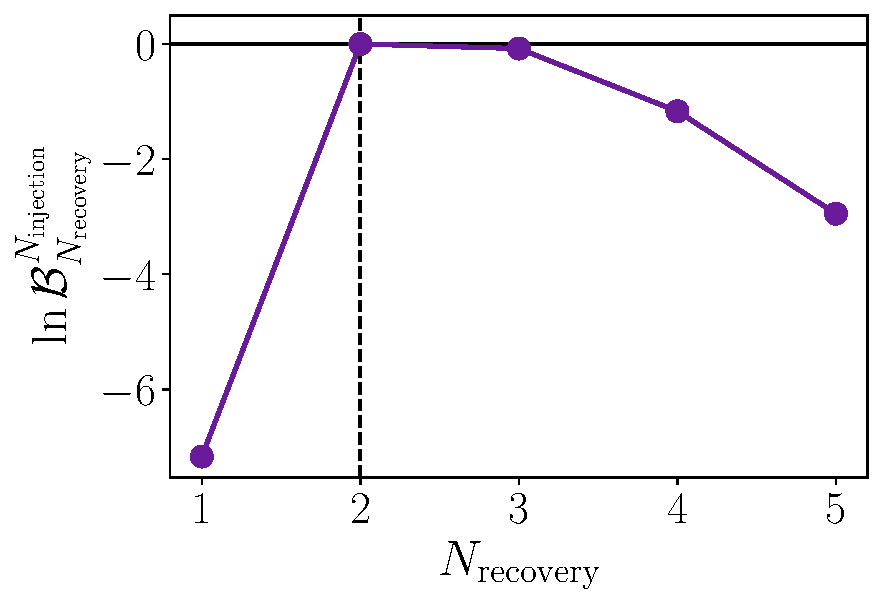
\includegraphics[width=0.99\linewidth]{Figures/senna_plot.pdf}
%       \end{figure}
%     \end{column}
%     \begin{column}{0.49\textwidth}
%       \centering
%       BW comparison figure
%     \end{column}
%   \end{columns}
% \end{frame}

\begin{frame}[allowframebreaks]{Evidence calculation: \textsc{harmonic}}

  Evidence $Z$ can be computed from posterior samples with \textsc{harmonic}~\cite{mcewen2023machinelearningassistedbayesian} with the \red{harmonic mean estimator}

  \begin{align*}
    \rho &\equiv \mathbb{E}_{P(\theta|d)}\left[\frac{1}{L(\theta)}\right] \\ 
    &= \int \diff \theta \frac{1}{\mathcal{L}(\theta)} P(\theta | d) \\
    &= \int \diff \theta \frac{1}{\mathcal{L}(\theta)} \frac{\mathcal{L}(\theta) \pi(\theta)}{Z} = \frac{1}{Z}
  \end{align*}

  Therefore, estimate $\rho$ with posterior samples:
  \begin{equation*}
    \hat{\rho} = \frac1N \sum_{i=1}^N \frac{1}{\mathcal{L}(\theta)}, \quad \theta_i \sim P(\theta|d)
  \end{equation*}

  Can be interpreted as importance sampling
  \begin{equation*}
    \rho = \int \diff \theta \frac1Z \frac{\pi(\theta)}{P(\theta | d)} P(\theta | d) \, ,
  \end{equation*}
  \textbf{but} with target = prior and sampling density = posterior. Therefore, importance sampling is inefficient -- how to solve?

  New proposal:
  \begin{align*}
    \rho &= \mathbb{E}_{P(\theta| d)}\left[ \frac{\varphi(\theta)}{\mathcal{L}(\theta)\pi(\theta)} \right] \\
    &= \int \mathrm{d}\theta \, \frac{\varphi(\theta)}{\mathcal{L}(\theta)\pi(\theta)} \, P(\theta| d) \\
    &= \int \mathrm{d}\theta \, \frac{\varphi(\theta)}{\mathcal{L}(\theta)\pi(\theta)} \, \frac{\mathcal{L}(\theta)\pi(\theta)}{Z} = \frac{1}{Z}
  \end{align*}

  Use the following estimator:
  \begin{equation*}
    \hat{\rho} = \frac{1}{N} \sum_{i=1}^N \frac{\varphi(\theta_i)}{\mathcal{L}(\theta_i)\pi(\theta_i)}, \quad \theta_i \sim P(\theta|d)
  \end{equation*}

  \vspace{5mm}
  Replace the target distribution $\pi$ with $\varphi$: only requirement is that it is normalized 
  
  \vspace{5mm}
  In practice, this can be achieved with a normalizing flow~\cite{polanska2024learnedharmonicmeanestimation}. \\
  
  \vspace{5mm}
  This has been verified to give accurate evidences (similar values as nested sampling) when GW posteriors are used~\cite{Polanska:2024zpn}. 
\end{frame}

\begin{frame}{\textsc{harmonic} with \textsc{jim}~\cite{Polanska:2024zpn}}
  \begin{figure}
    \centering
    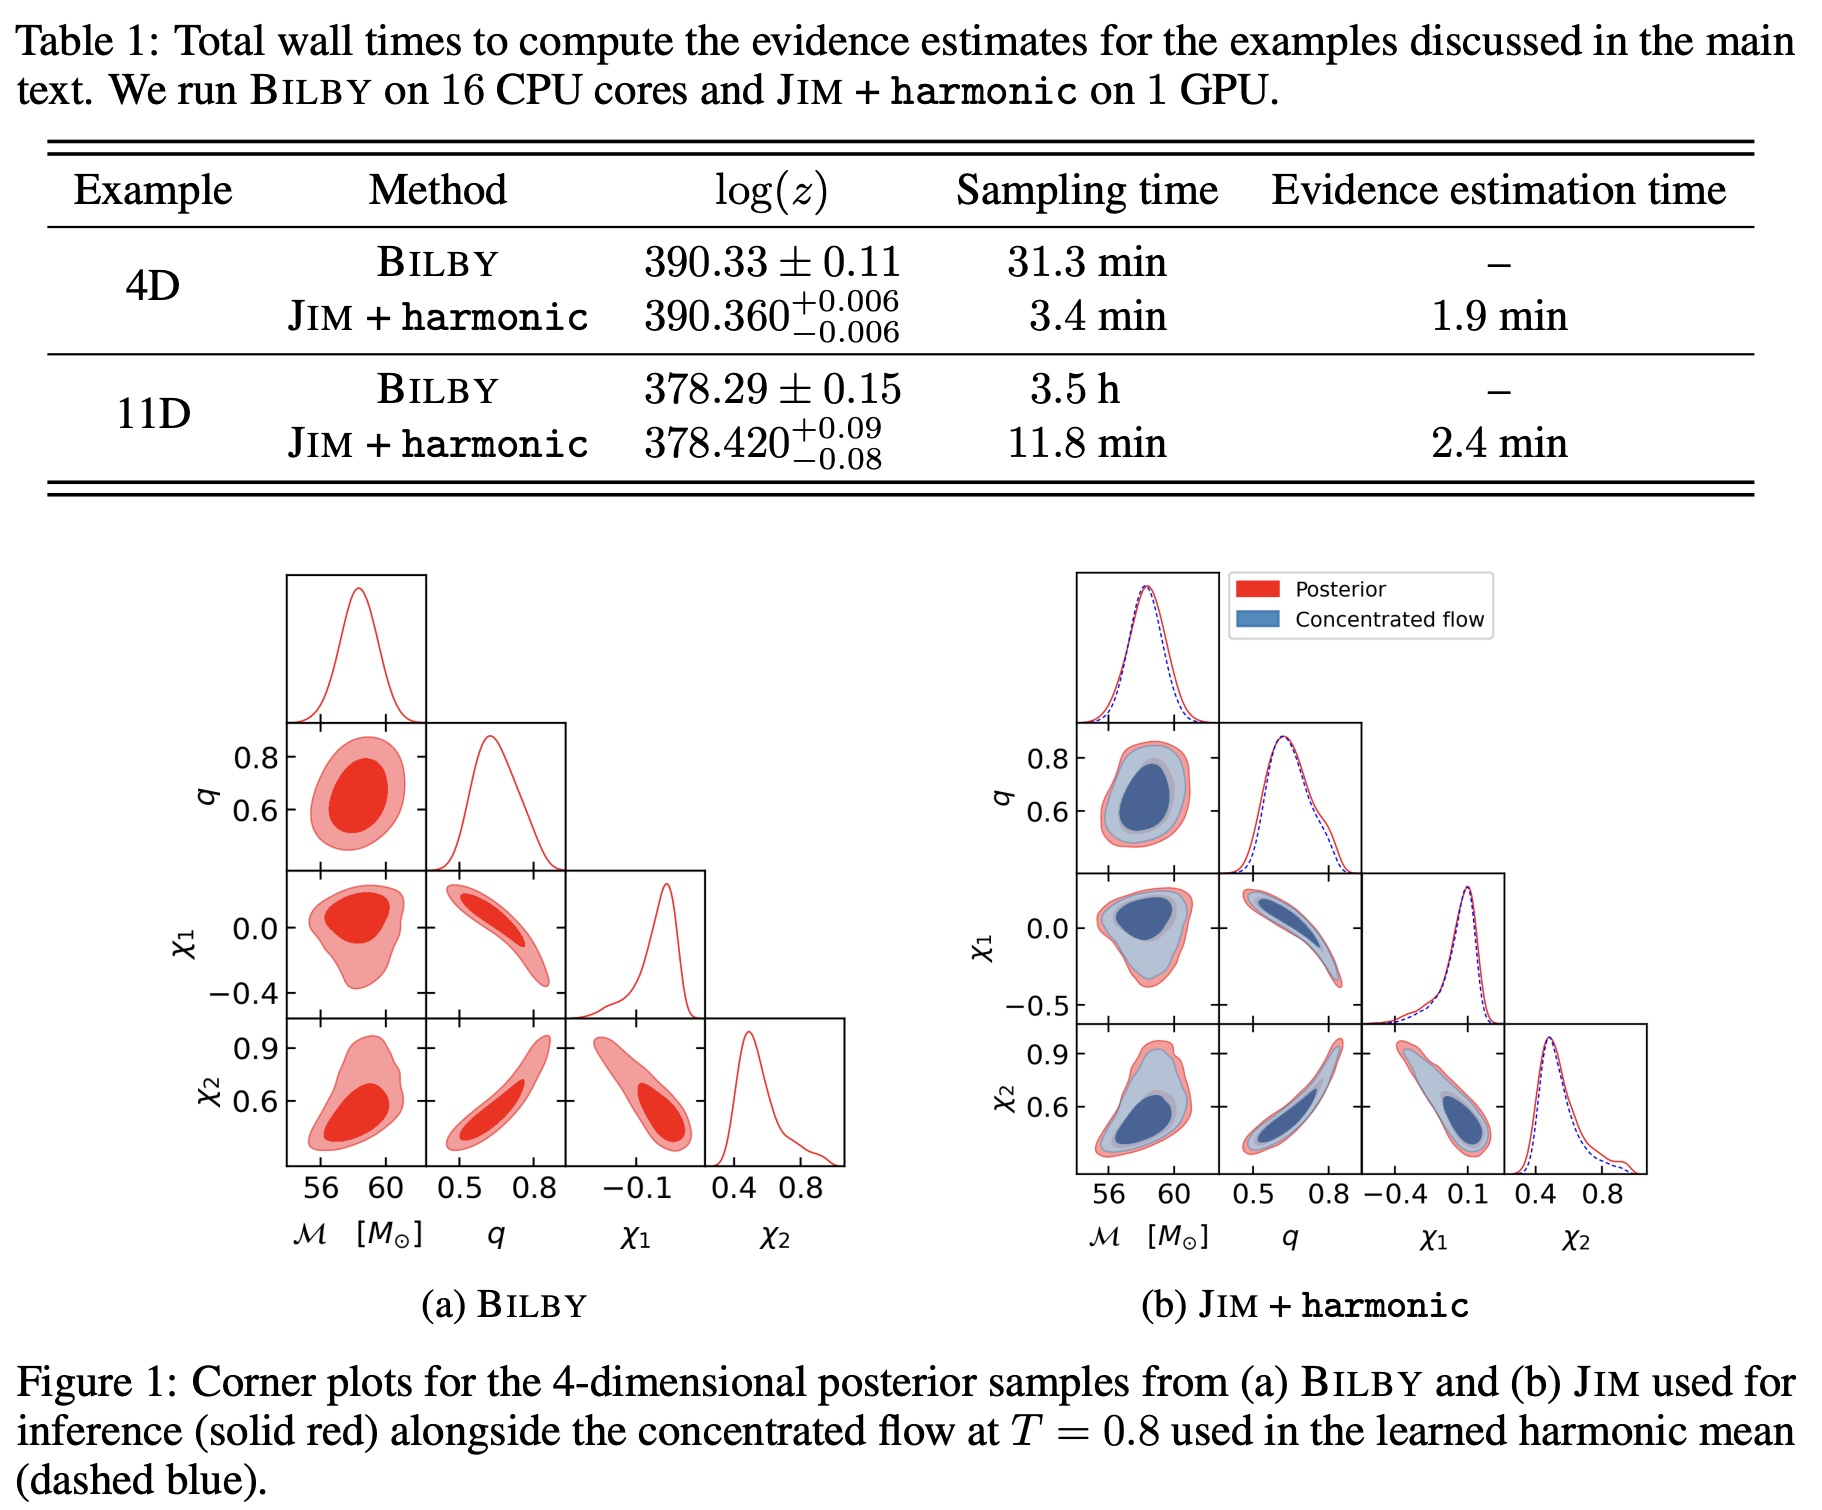
\includegraphics[scale=0.275]{Figures/polanska.jpg}
  \end{figure}
  
\end{frame}

\begin{frame}{BNS in ET-$\Delta$ example: all parameters}
  \vspace{-3mm}
  \begin{figure}
    \centering
    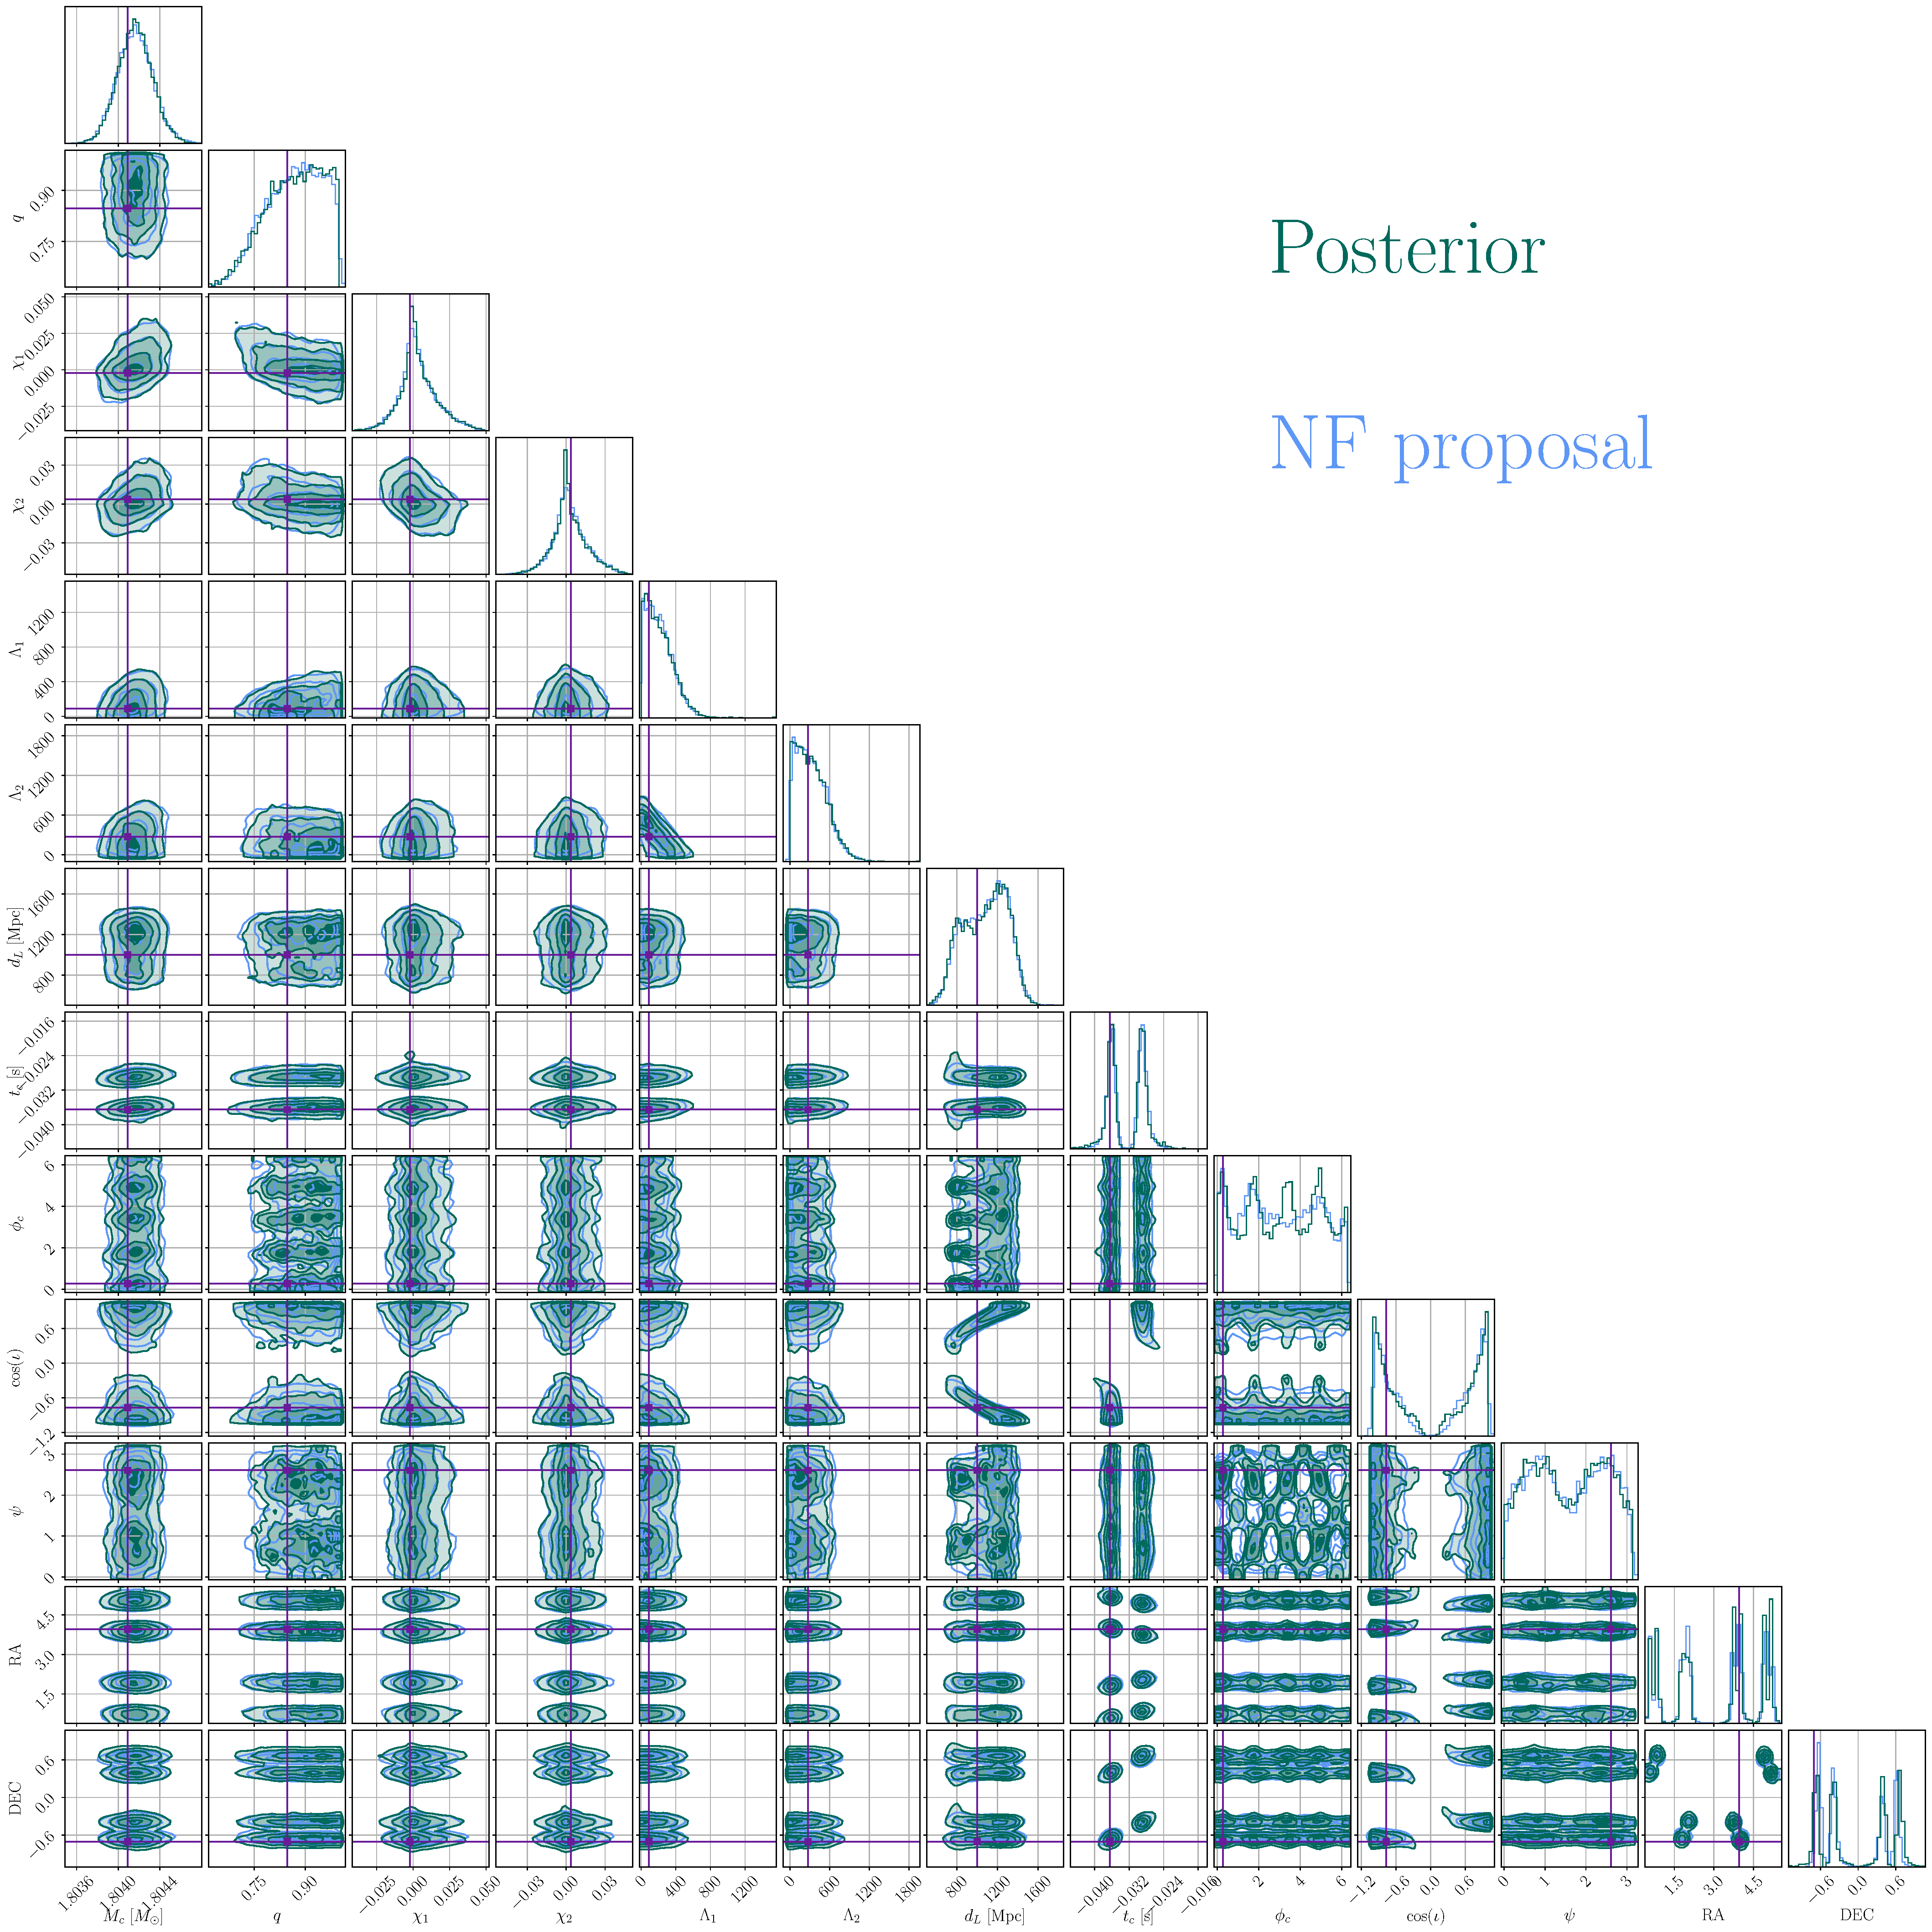
\includegraphics[scale=0.1125]{Figures/corner_plot_big.pdf}
  \end{figure}
\end{frame}

\begin{frame}{Overlapping signals: all parameters signal A}
  \vspace{-3mm}
  \begin{figure}
    \centering
    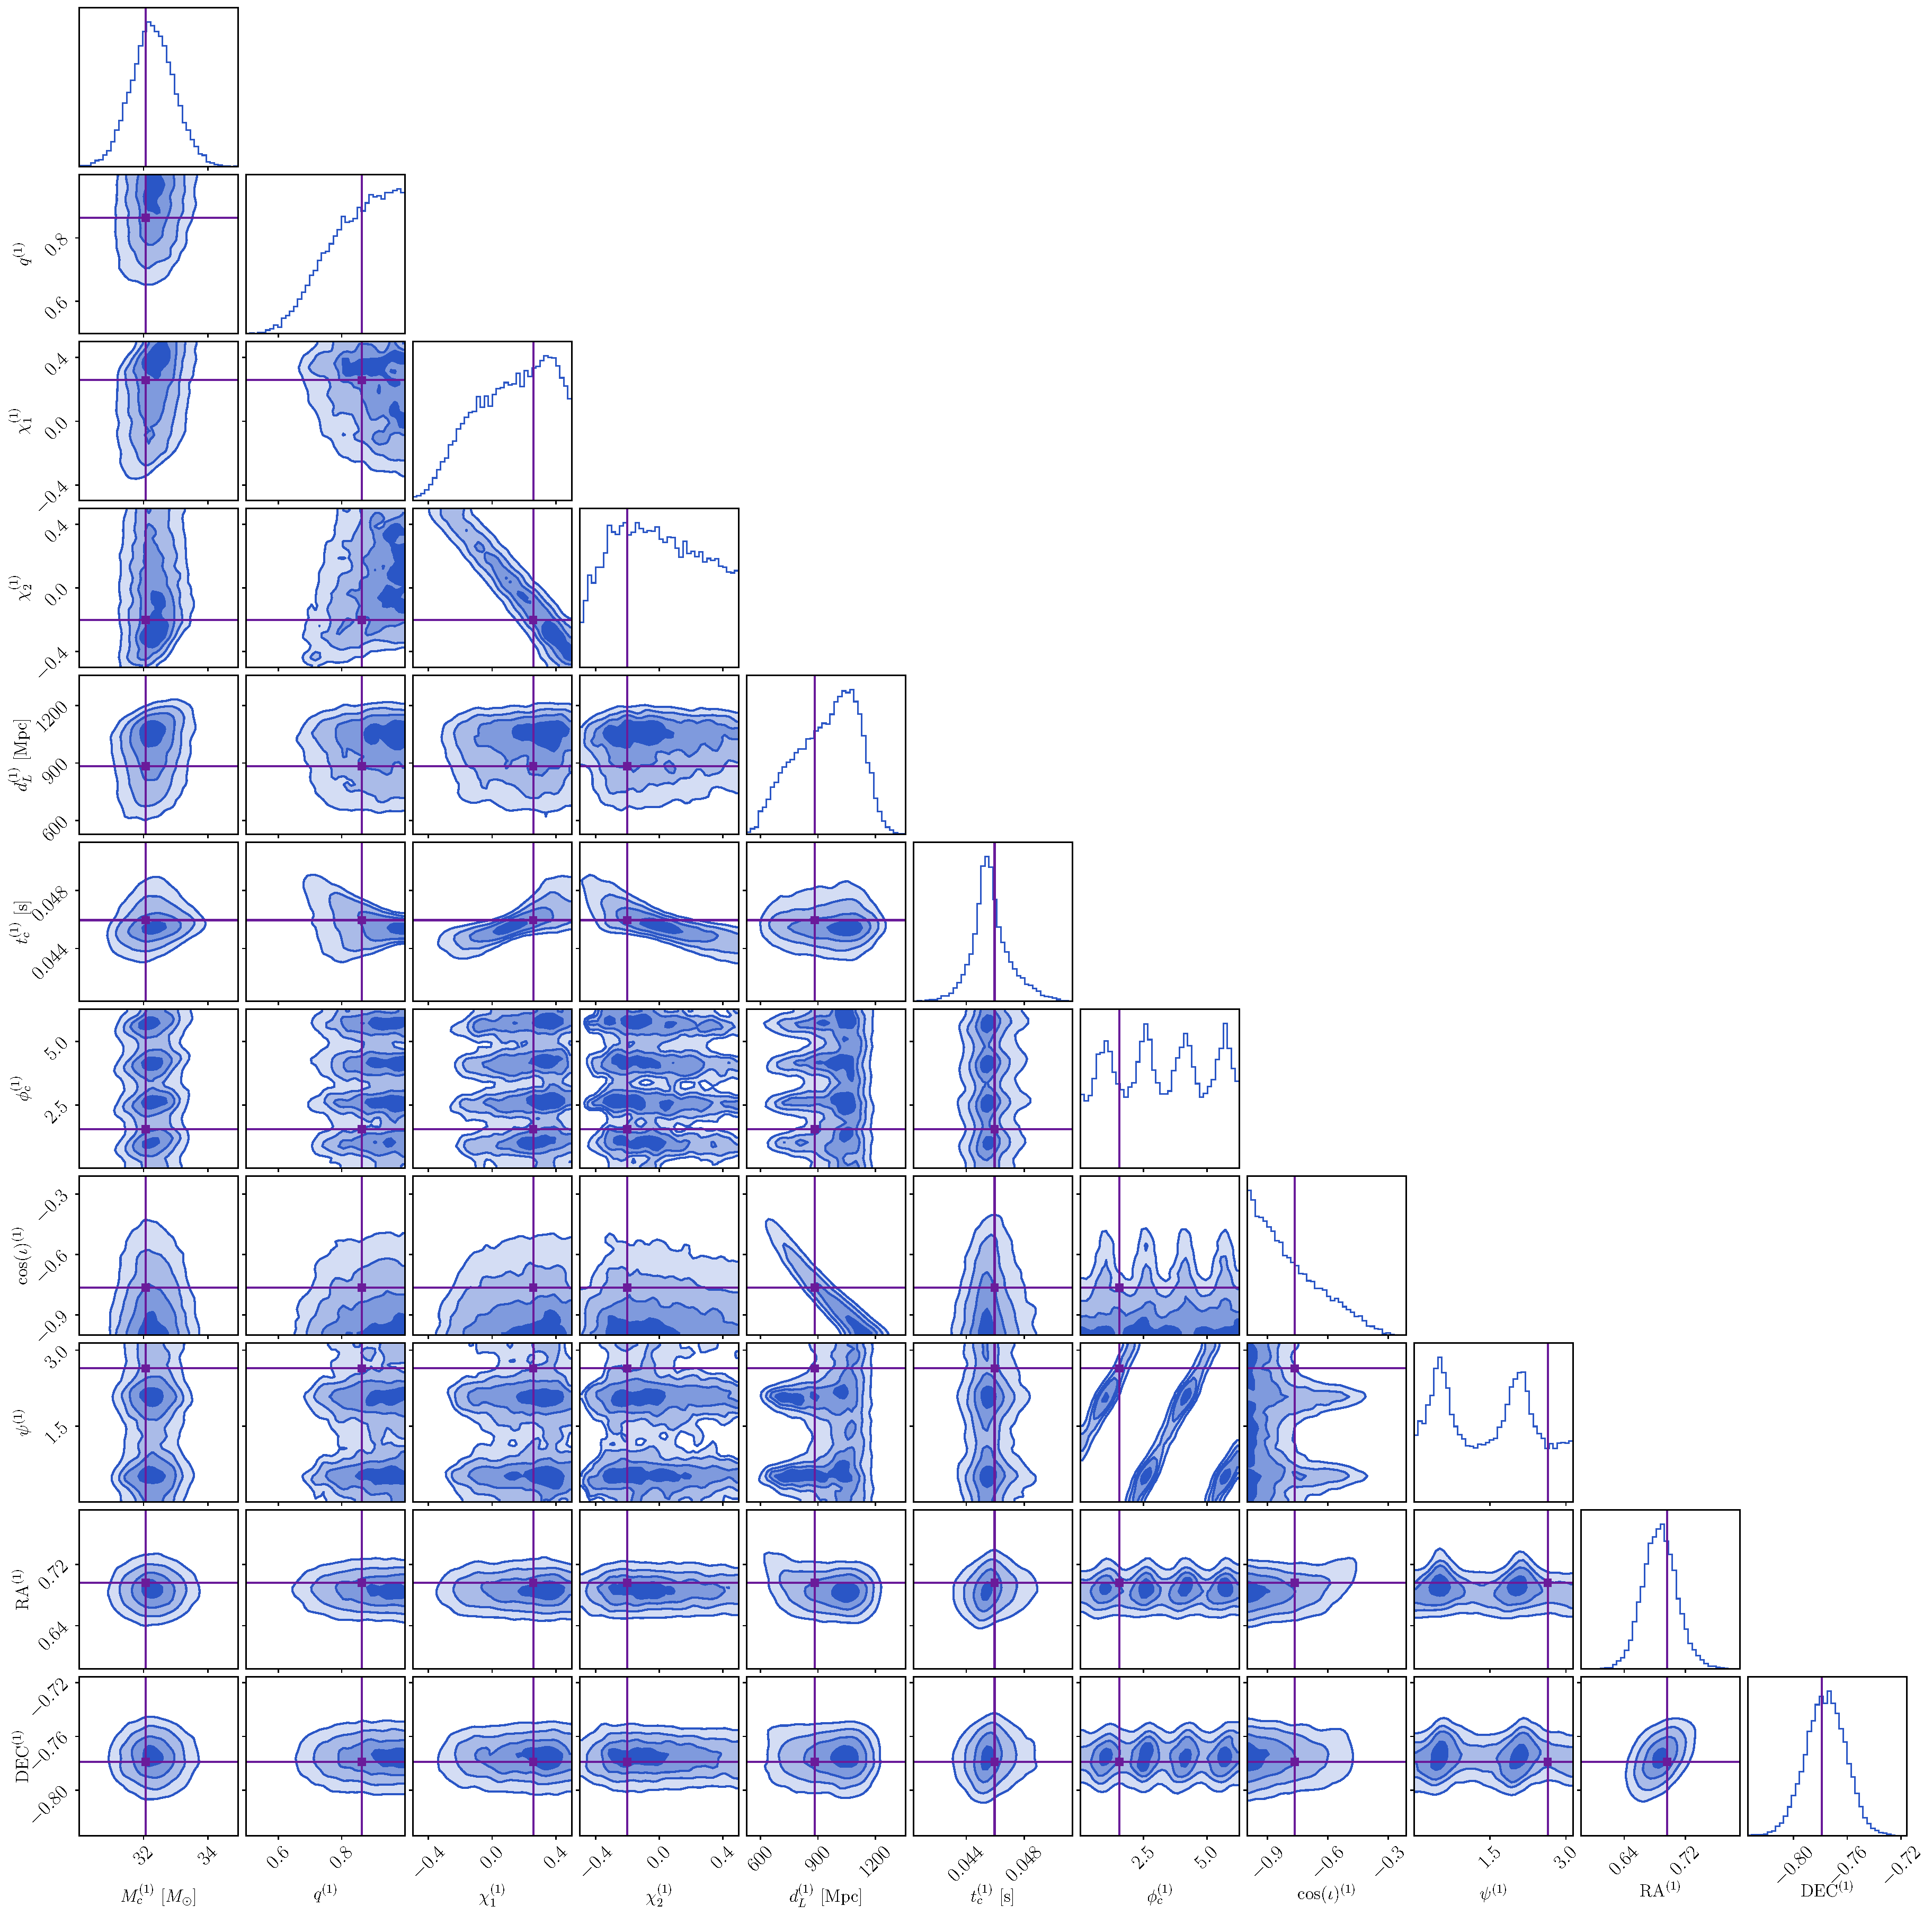
\includegraphics[scale=0.1325]{Figures/OS_injection_139_v2_1_cornerplot_all.pdf}
  \end{figure}
\end{frame}

\begin{frame}{Overlapping signals: all parameters signal B}
  \vspace{-3mm}
  \begin{figure}
    \centering
    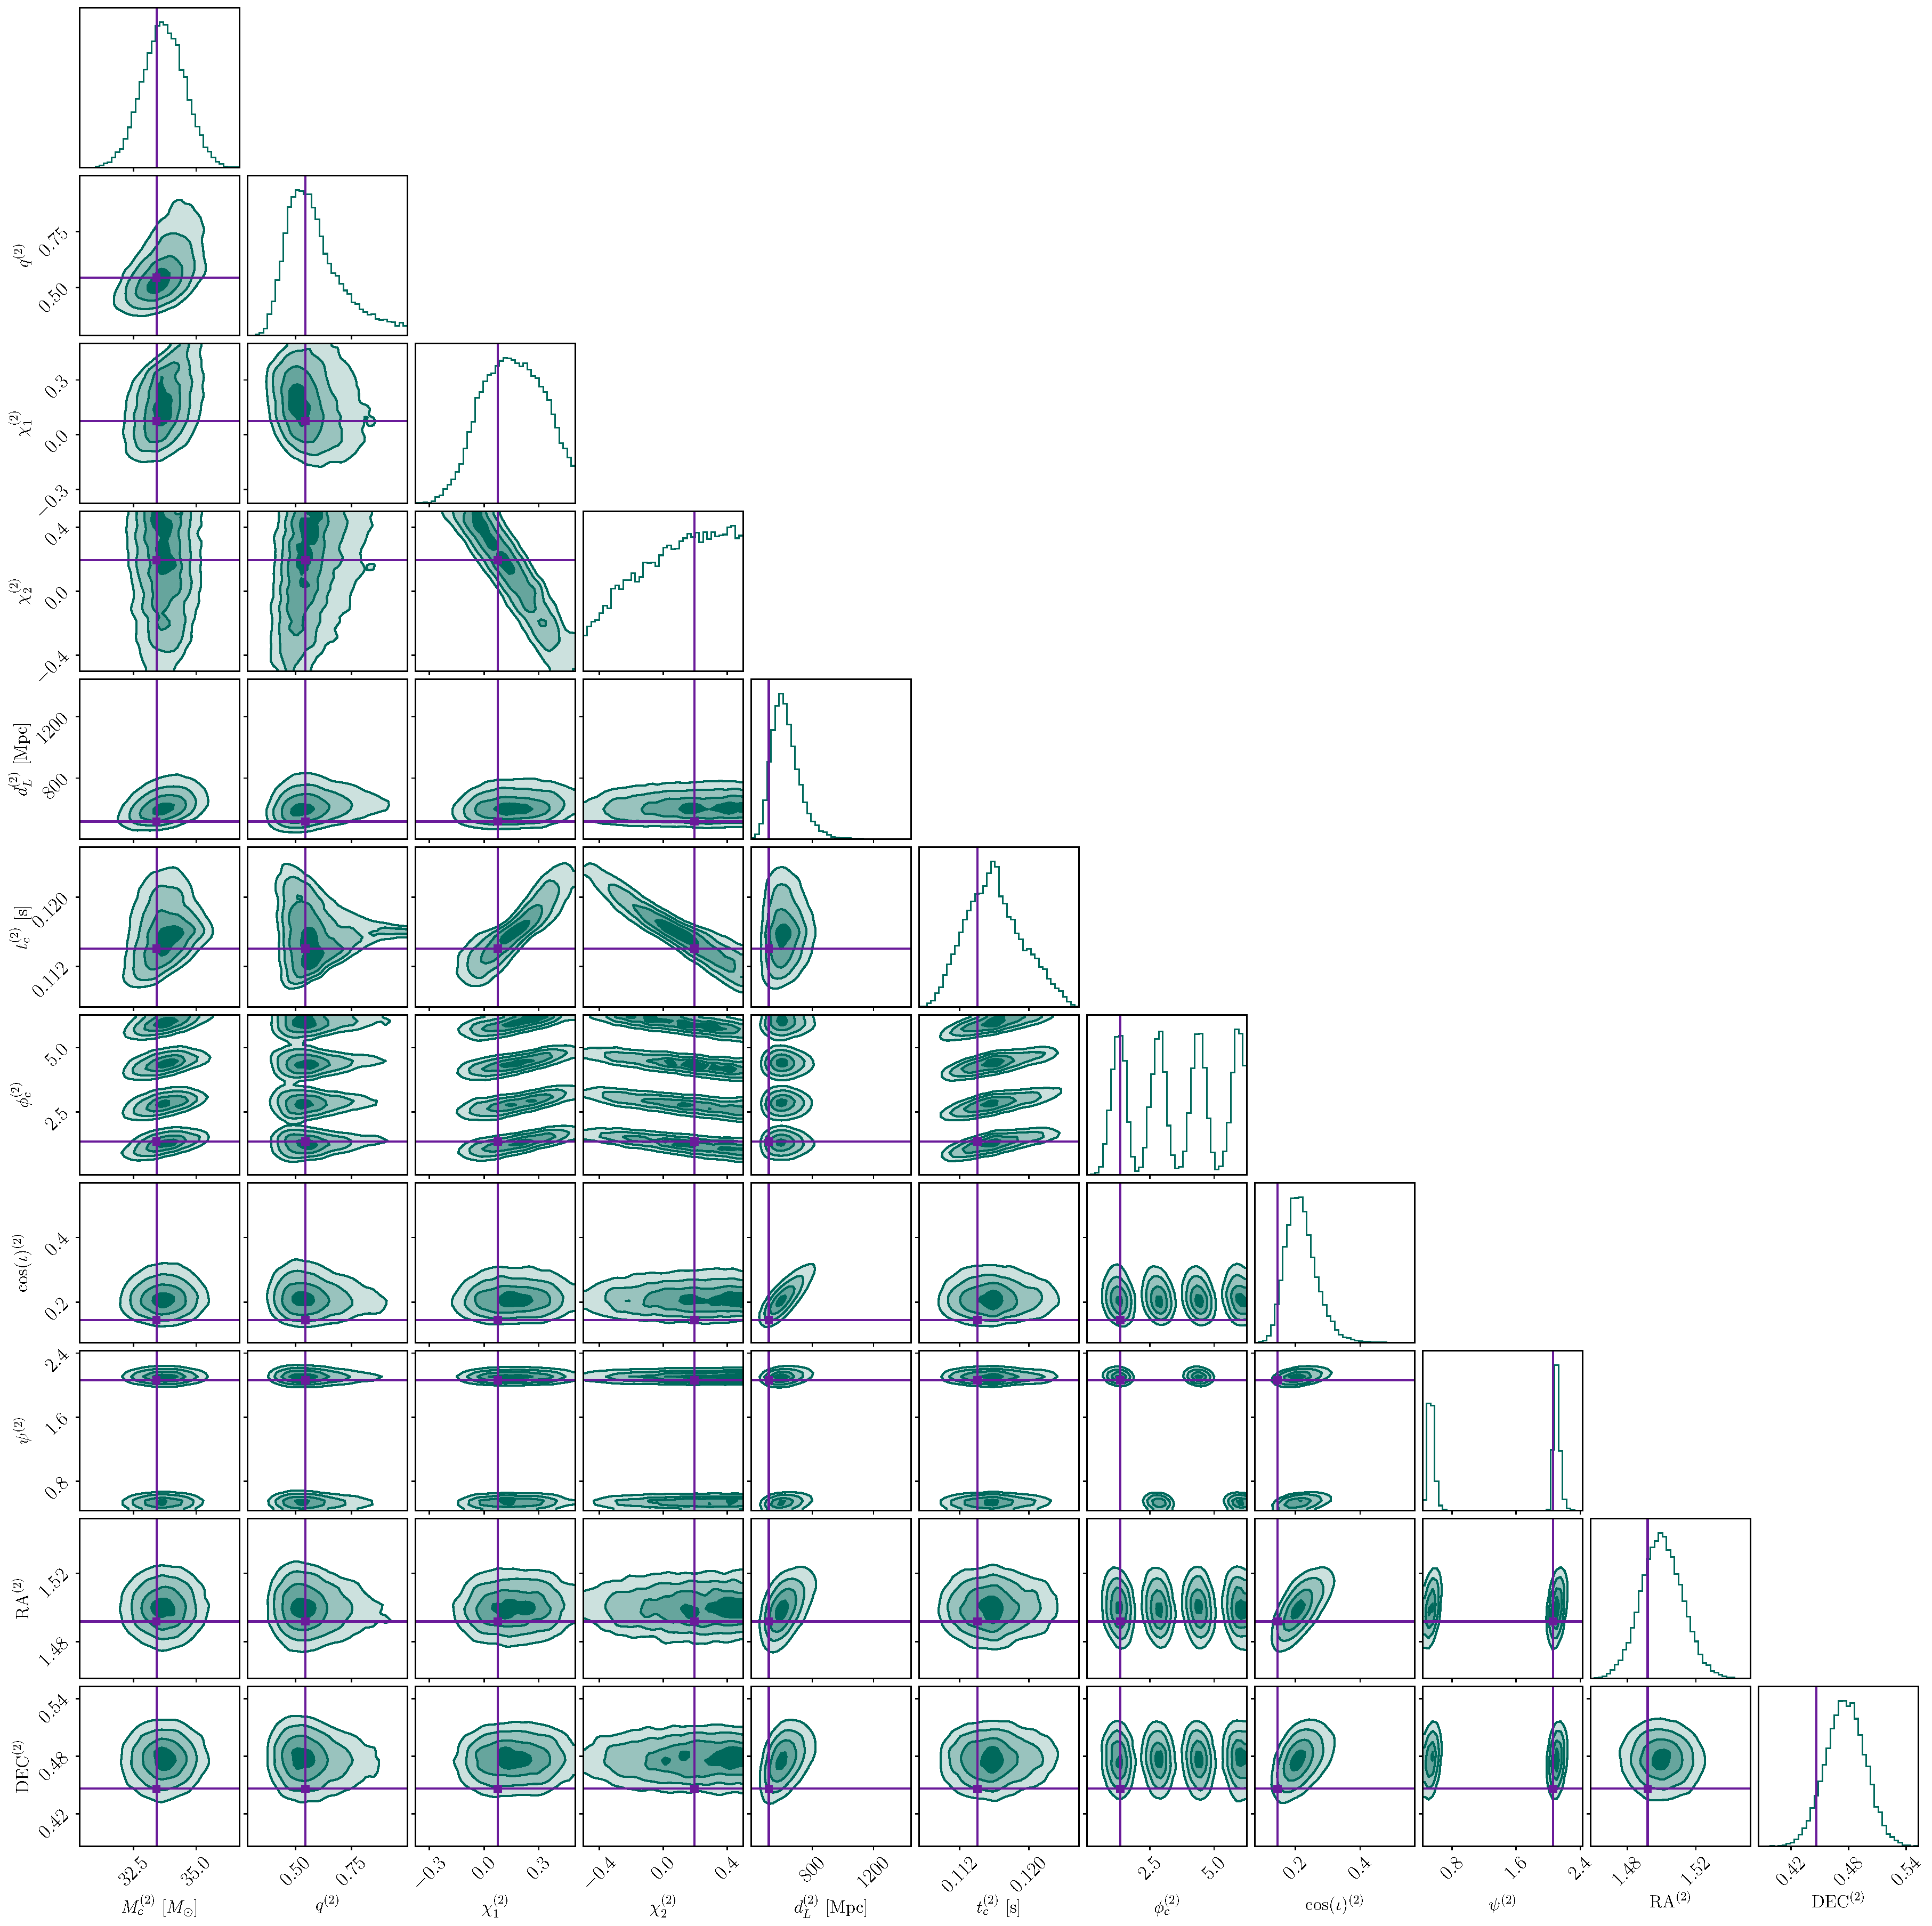
\includegraphics[scale=0.1325]{Figures/OS_injection_139_v2_2_cornerplot_all.pdf}
  \end{figure}
\end{frame}

\begin{frame}{Equation of state O5 projection with 20 BNS: EOS}

  \vspace{-2mm}
  \begin{itemize}
    \item \textbf{\jaxthree{Purple}}: target
    \item \textbf{\red{Red}}: posterior EOS samples (\textbf{black}: maximum log posterior)
  \end{itemize}

  \begin{figure}
    \centering
    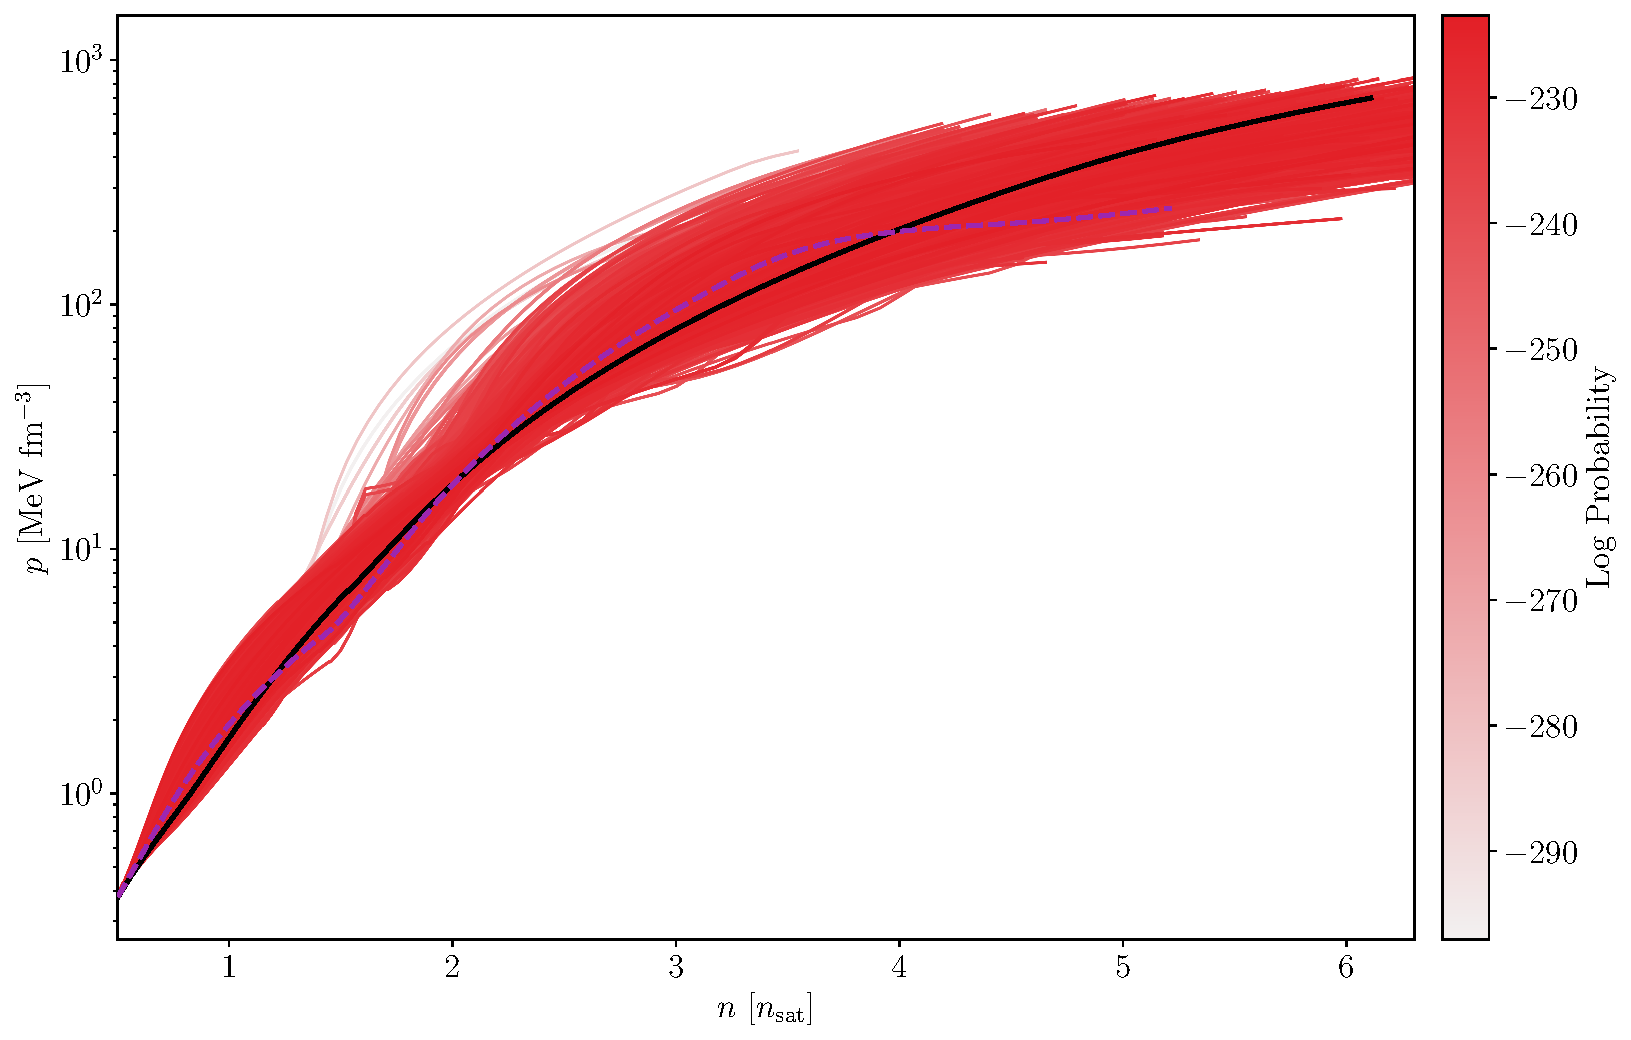
\includegraphics[scale=0.40]{Figures/postprocessing_EOS.pdf}
  \end{figure}
\end{frame}

\begin{frame}{Equation of state O5 projection with 20 BNS: NS}
  \begin{figure}
    \centering
    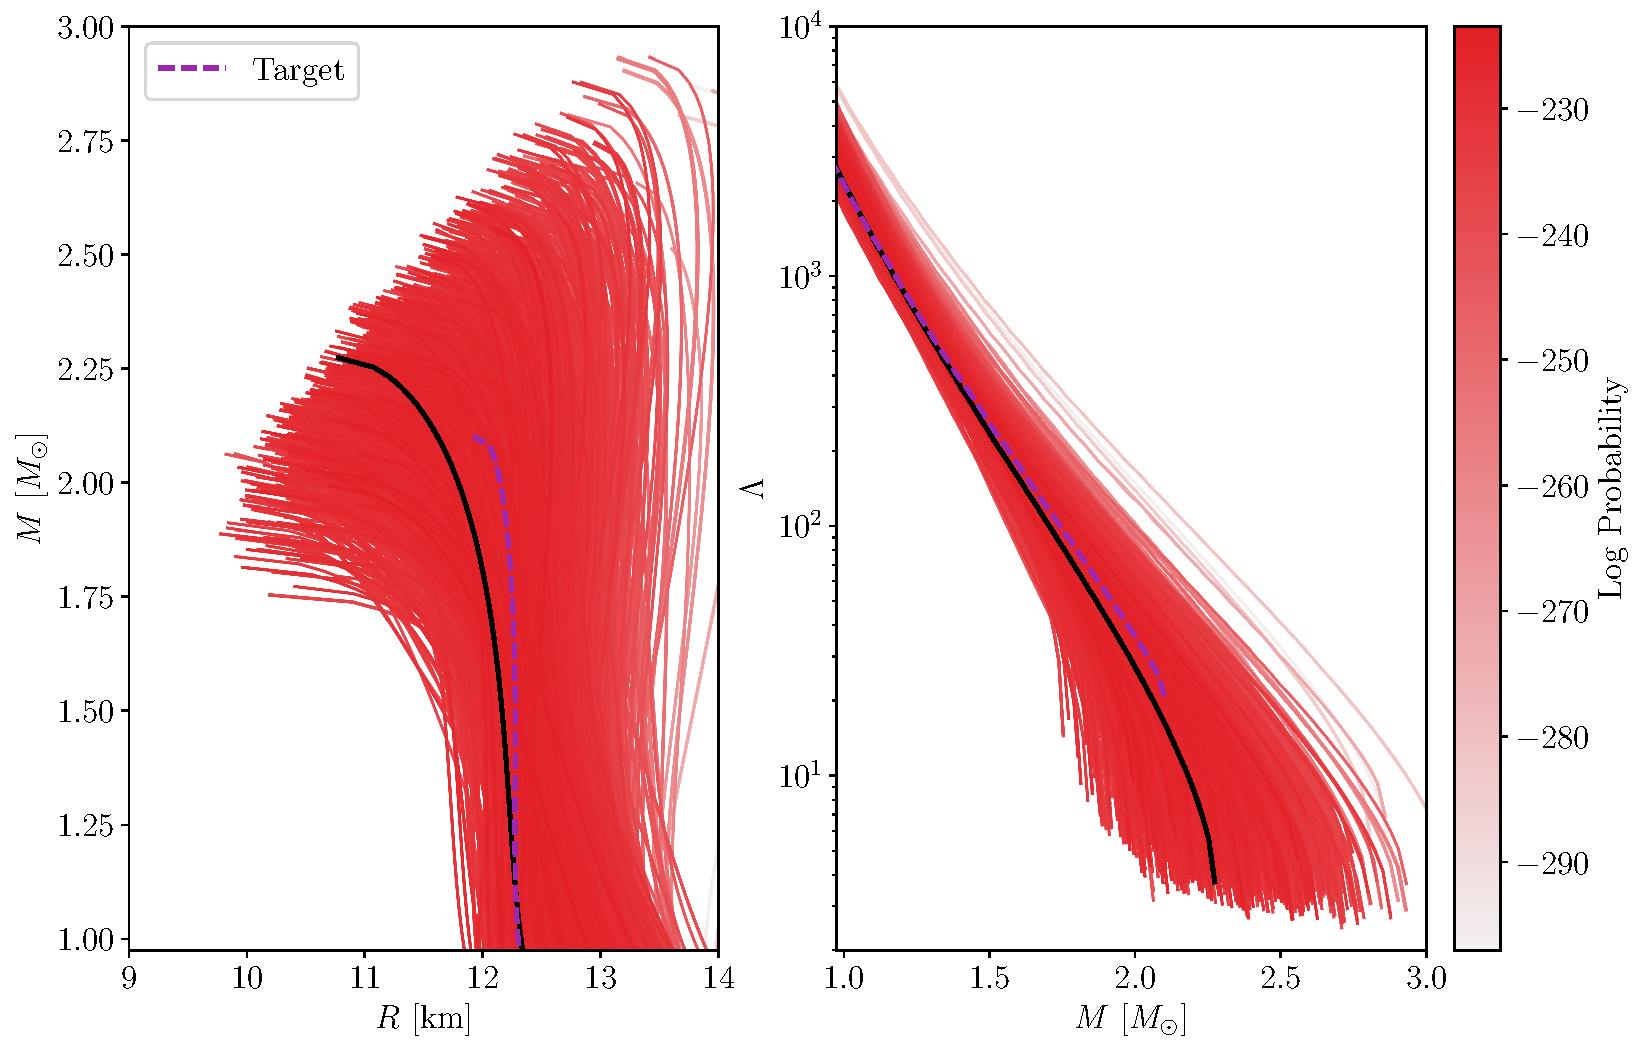
\includegraphics[scale=0.40]{Figures/postprocessing_NS.pdf}
  \end{figure}
\end{frame}


\end{document}